O processo de automação aplicou as flags apresentadas na Tabela \ref{tab:flags}, à exceção das que se encontram a itálico, a todos os contratos adicionadas à base de dados, até ao início de julho. Porém, por motivos de consistência, só se analisaram os contratos celebrados até ao dia 1 de maio do presente ano civil, tal como foi estabelecido no Capítulo \ref{ch:variables}. A flag RF1 foi aplicada, manualmente, a todos os ajustes diretos celebrados ao longo do mesmo período de tempo considerado.


\begin{table}[ht]
	\centering
	\renewcommand{\arraystretch}{1.2}
	\setlength{\tabcolsep}{15pt}
	\resizebox{\textwidth}{!}{
		\begin{tabular}{lllll}
			\hline
			\rowcolor[HTML]{EFEFEF} 
			\multicolumn{1}{c}{\cellcolor[HTML]{EFEFEF}\textbf{Flag}} & \multicolumn{4}{c}{\cellcolor[HTML]{EFEFEF}\textbf{Descrição}}                                               \\ \hline
			\textit{RF1}                                                       & \multicolumn{4}{l}{\textit{Verificação dos preços contratuais para ajustes diretos.}}                                 \\ \hline
			RF2                                                       & \multicolumn{4}{l}{Comparação entre o preço base e o preço total efetivo.}             \\
			RF3                                                       & \multicolumn{4}{l}{Análise da publicação de anúncios em datas não convencionais.}                            \\
			R003                                                      & \multicolumn{4}{l}{Análise do prazo de apresentação de propostas.}                                           \\
			R017                                                      & \multicolumn{4}{l}{Análise do preço contratual, por grupo de CPV.}                    \\
			R018                                                      & \multicolumn{4}{l}{Análise de concursos públicos com uma entidade concorrente.}                              \\
			R019                                                      & \multicolumn{4}{l}{Análise do número de entidades concorrentes.}                       \\ \hline
			{\textit{R031}}                                       & \multicolumn{4}{l}{{ \textit{Comparação entre o preço base e o preço contratual.}}} \\
			{\textit{R051}}                                       & \multicolumn{4}{l}{{ \textit{Análise da concentração de mercado.}}}                                       \\ \hline
		\end{tabular}%
	}
	\caption{Conjunto de flags desenvolvidas.}
	\label{tab:flags}
\end{table}


A partir da Tabela \ref{final1} podem ser repescados os números relativos a ajustes diretos e concursos públicos celebrados, bem como número de contratos inconformes e/ou sinalizados, e respetiva percentagem face à totalidade de contratos celebrados, para cada uma das \textit{flags} aplicadas ao longo deste processo. Do conjunto de \textit{flags} apresentadas, destacam-se a R017, R018 e R019, com uma percentagem de contratos sinalizados de 21\%, 19.9\% e 23.5\%, respetivamente. 


\begin{table}[ht]
	\centering
	\renewcommand{\arraystretch}{1.5}
	\setlength{\tabcolsep}{10pt}
	\resizebox{\textwidth}{!}{
		\begin{tabular}{lclcccccc}
			\toprule[2px]
			\textbf{Tipo de Procedimento}                                                       & \multicolumn{2}{c}{Ajuste Direto} & \multicolumn{6}{c}{Concurso Público}       \\ \hline
			\textbf{Total de concursos}                                                         & \multicolumn{2}{c}{526860}        & \multicolumn{6}{c}{128422}                 \\ \midrule[1.5px]
			\textbf{Flag}                                                                       & \multicolumn{2}{c}{RF1}           & RF2 & RF3   & R003 & R017  & R018  & R019  \\ \hline
			\textbf{\begin{tabular}[c]{@{}l@{}}Número de \\ contratos sinalizados\end{tabular}} & \multicolumn{2}{c}{16910}         & 0   & 11958 & 4751 & 27261 & 25853 & 30576 \\ \hline
			\textbf{Percentagem \%}                                                             & \multicolumn{2}{c}{3.1}           & 0   & 9.2   & 3.7  & 21    & 19.9  & 23.5  \\ \bottomrule[1.5px]
		\end{tabular}%
	}
	\caption{Número de contratos sinalizados detetados para cada indicador construído e respetiva percentagem relativa ao número total de contratos celebrados.}
	\label{final1}
\end{table}


Nas Figuras \ref{final2}, \ref{final3}, \ref{final4}, \ref{final5} e \ref{final6} pode-se compreender a evolução do número de contratos sinalizados e a respetiva percentagem por ano e para cada \textit{flag}. À exceção das \textit{flags} RF3 e R018, todas as restantes sinalizam um maior número de inconformidades, em relação ao definido nas respetivas flags, no ano de 2023. Esta observação presume-se estar associada ao facto de ter sido neste ano civil onde se registou um maior número de contratos celebrados, tal como se contemplou na Figura \ref{fig:precocps1}.



\begin{figure}[H]
	\centering
	\begin{minipage}{.44\linewidth}
		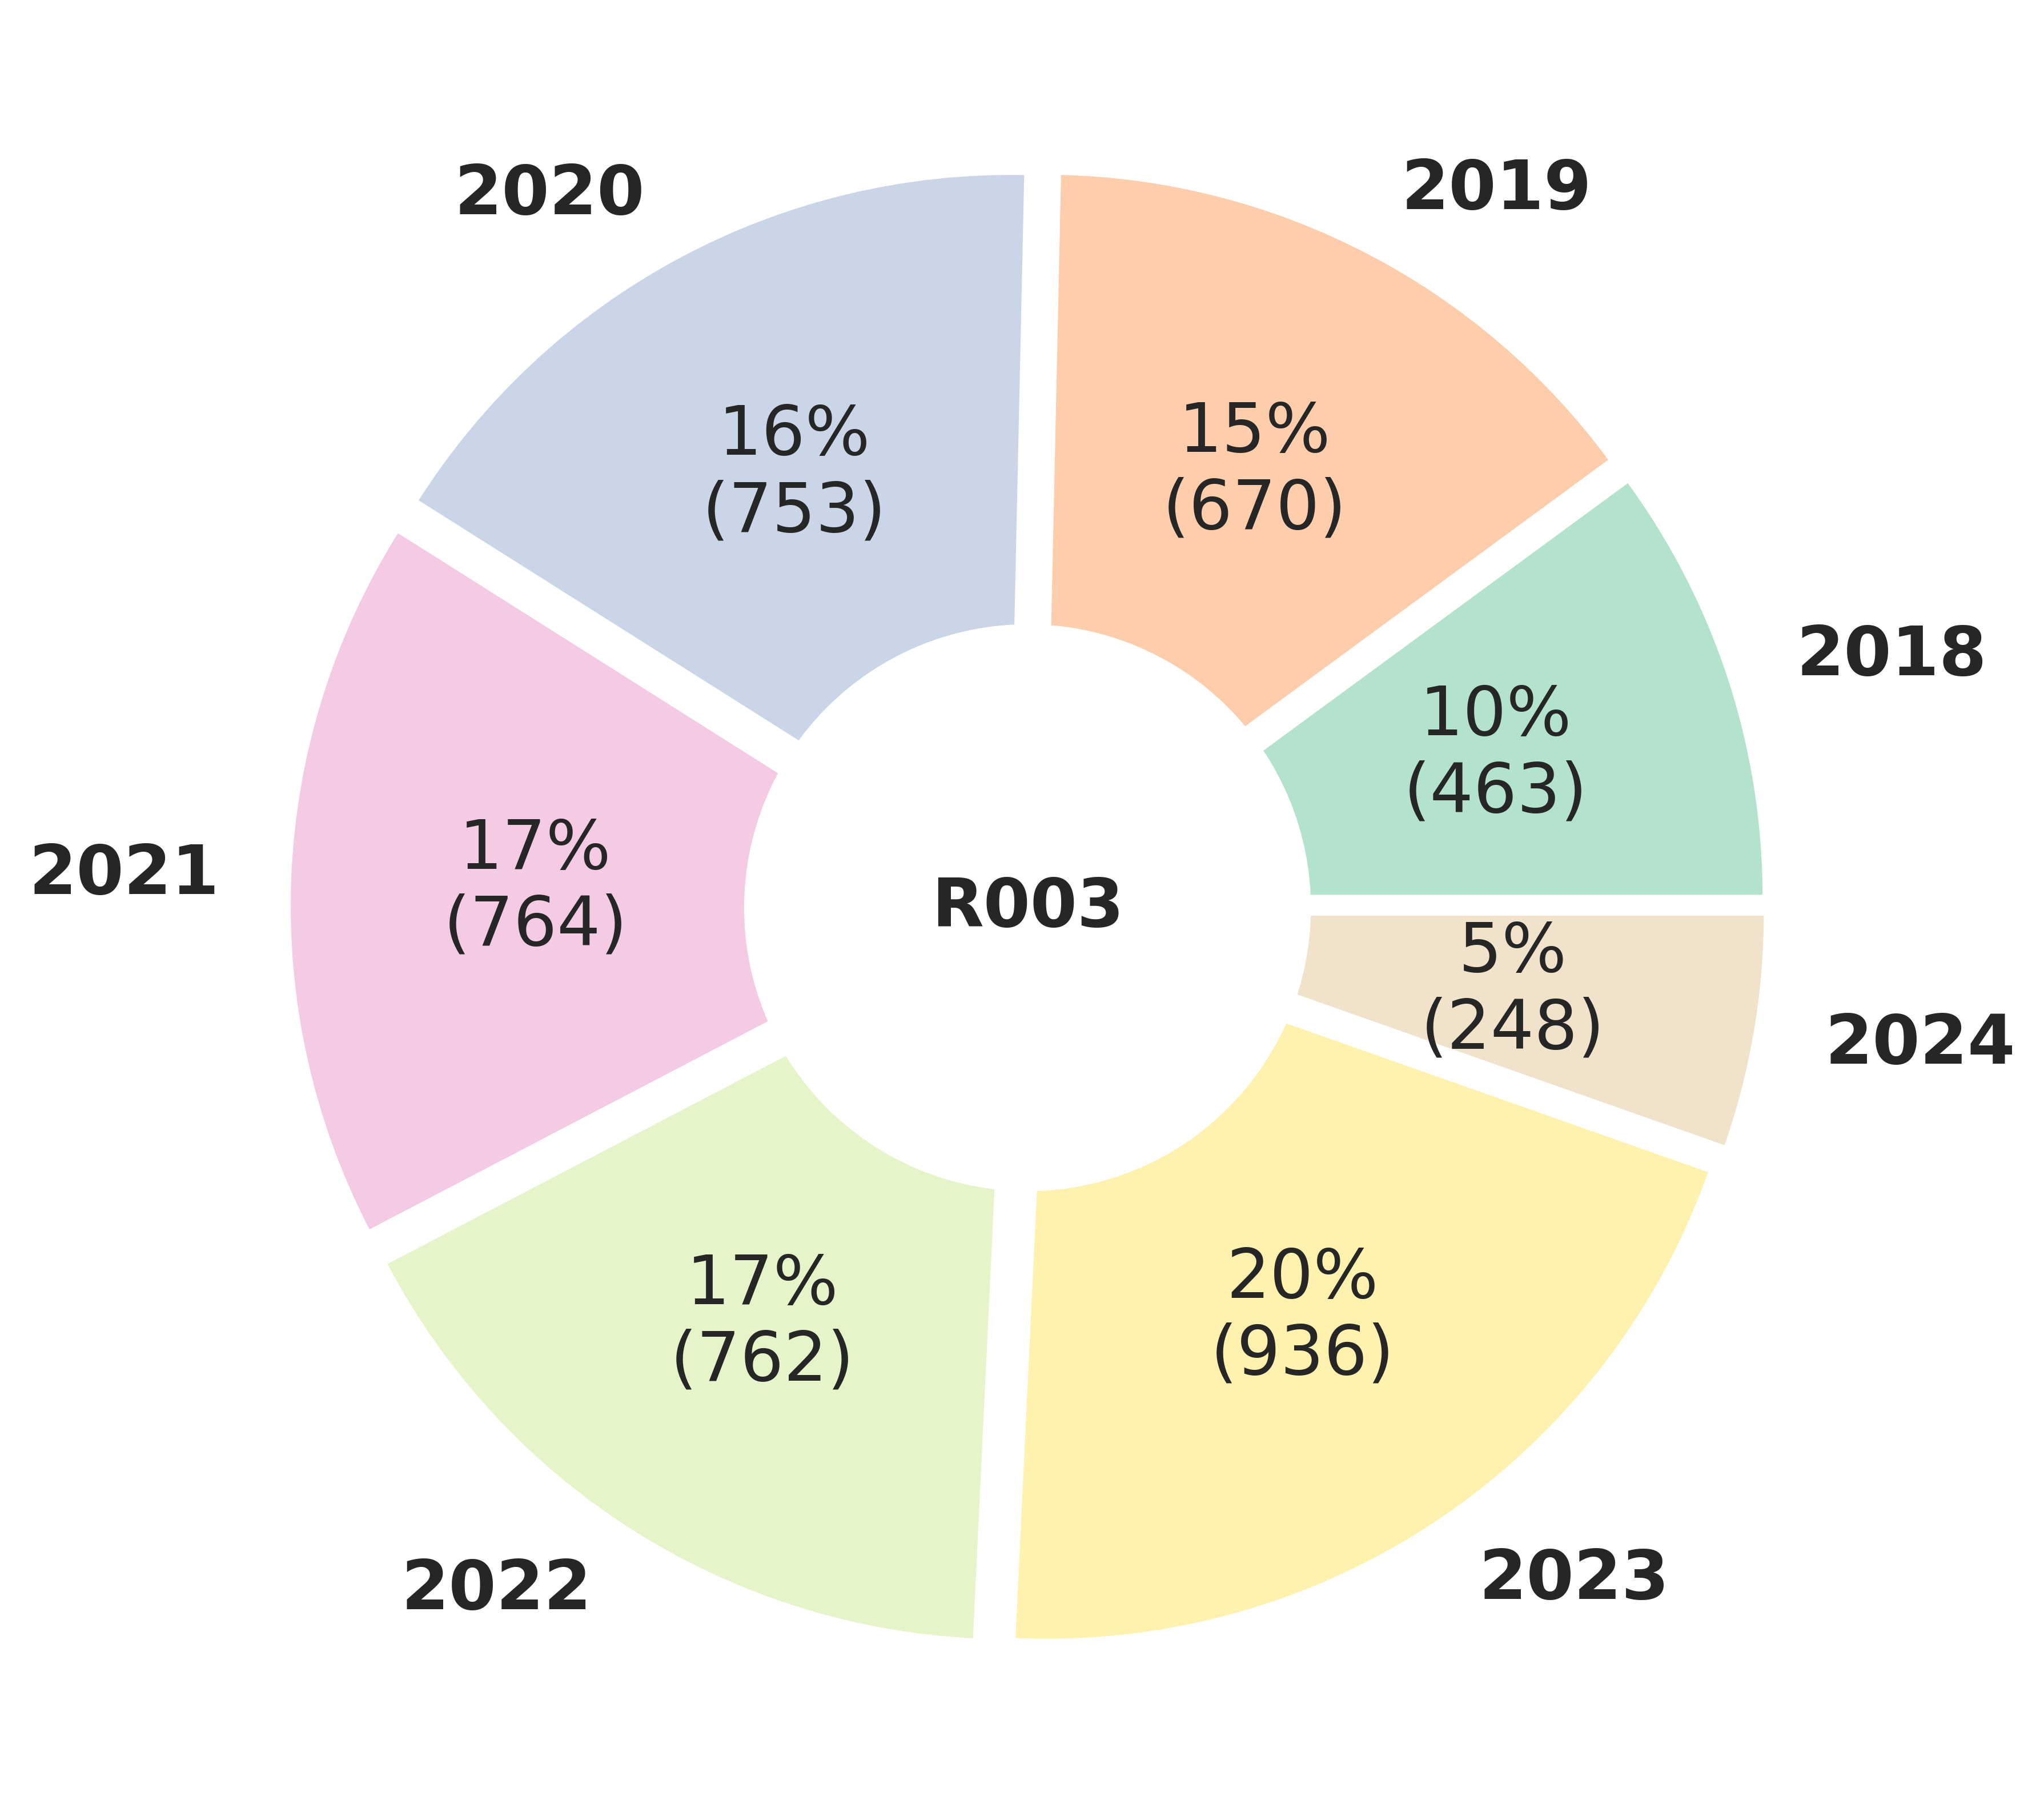
\includegraphics[width=\linewidth]{imagens/final/circle_R003.png}
		\caption{Número de contratos sinalizados para o indicador R003, por ano.}
		\label{final2}
	\end{minipage}
	\hfill
	\begin{minipage}{.44\linewidth}
		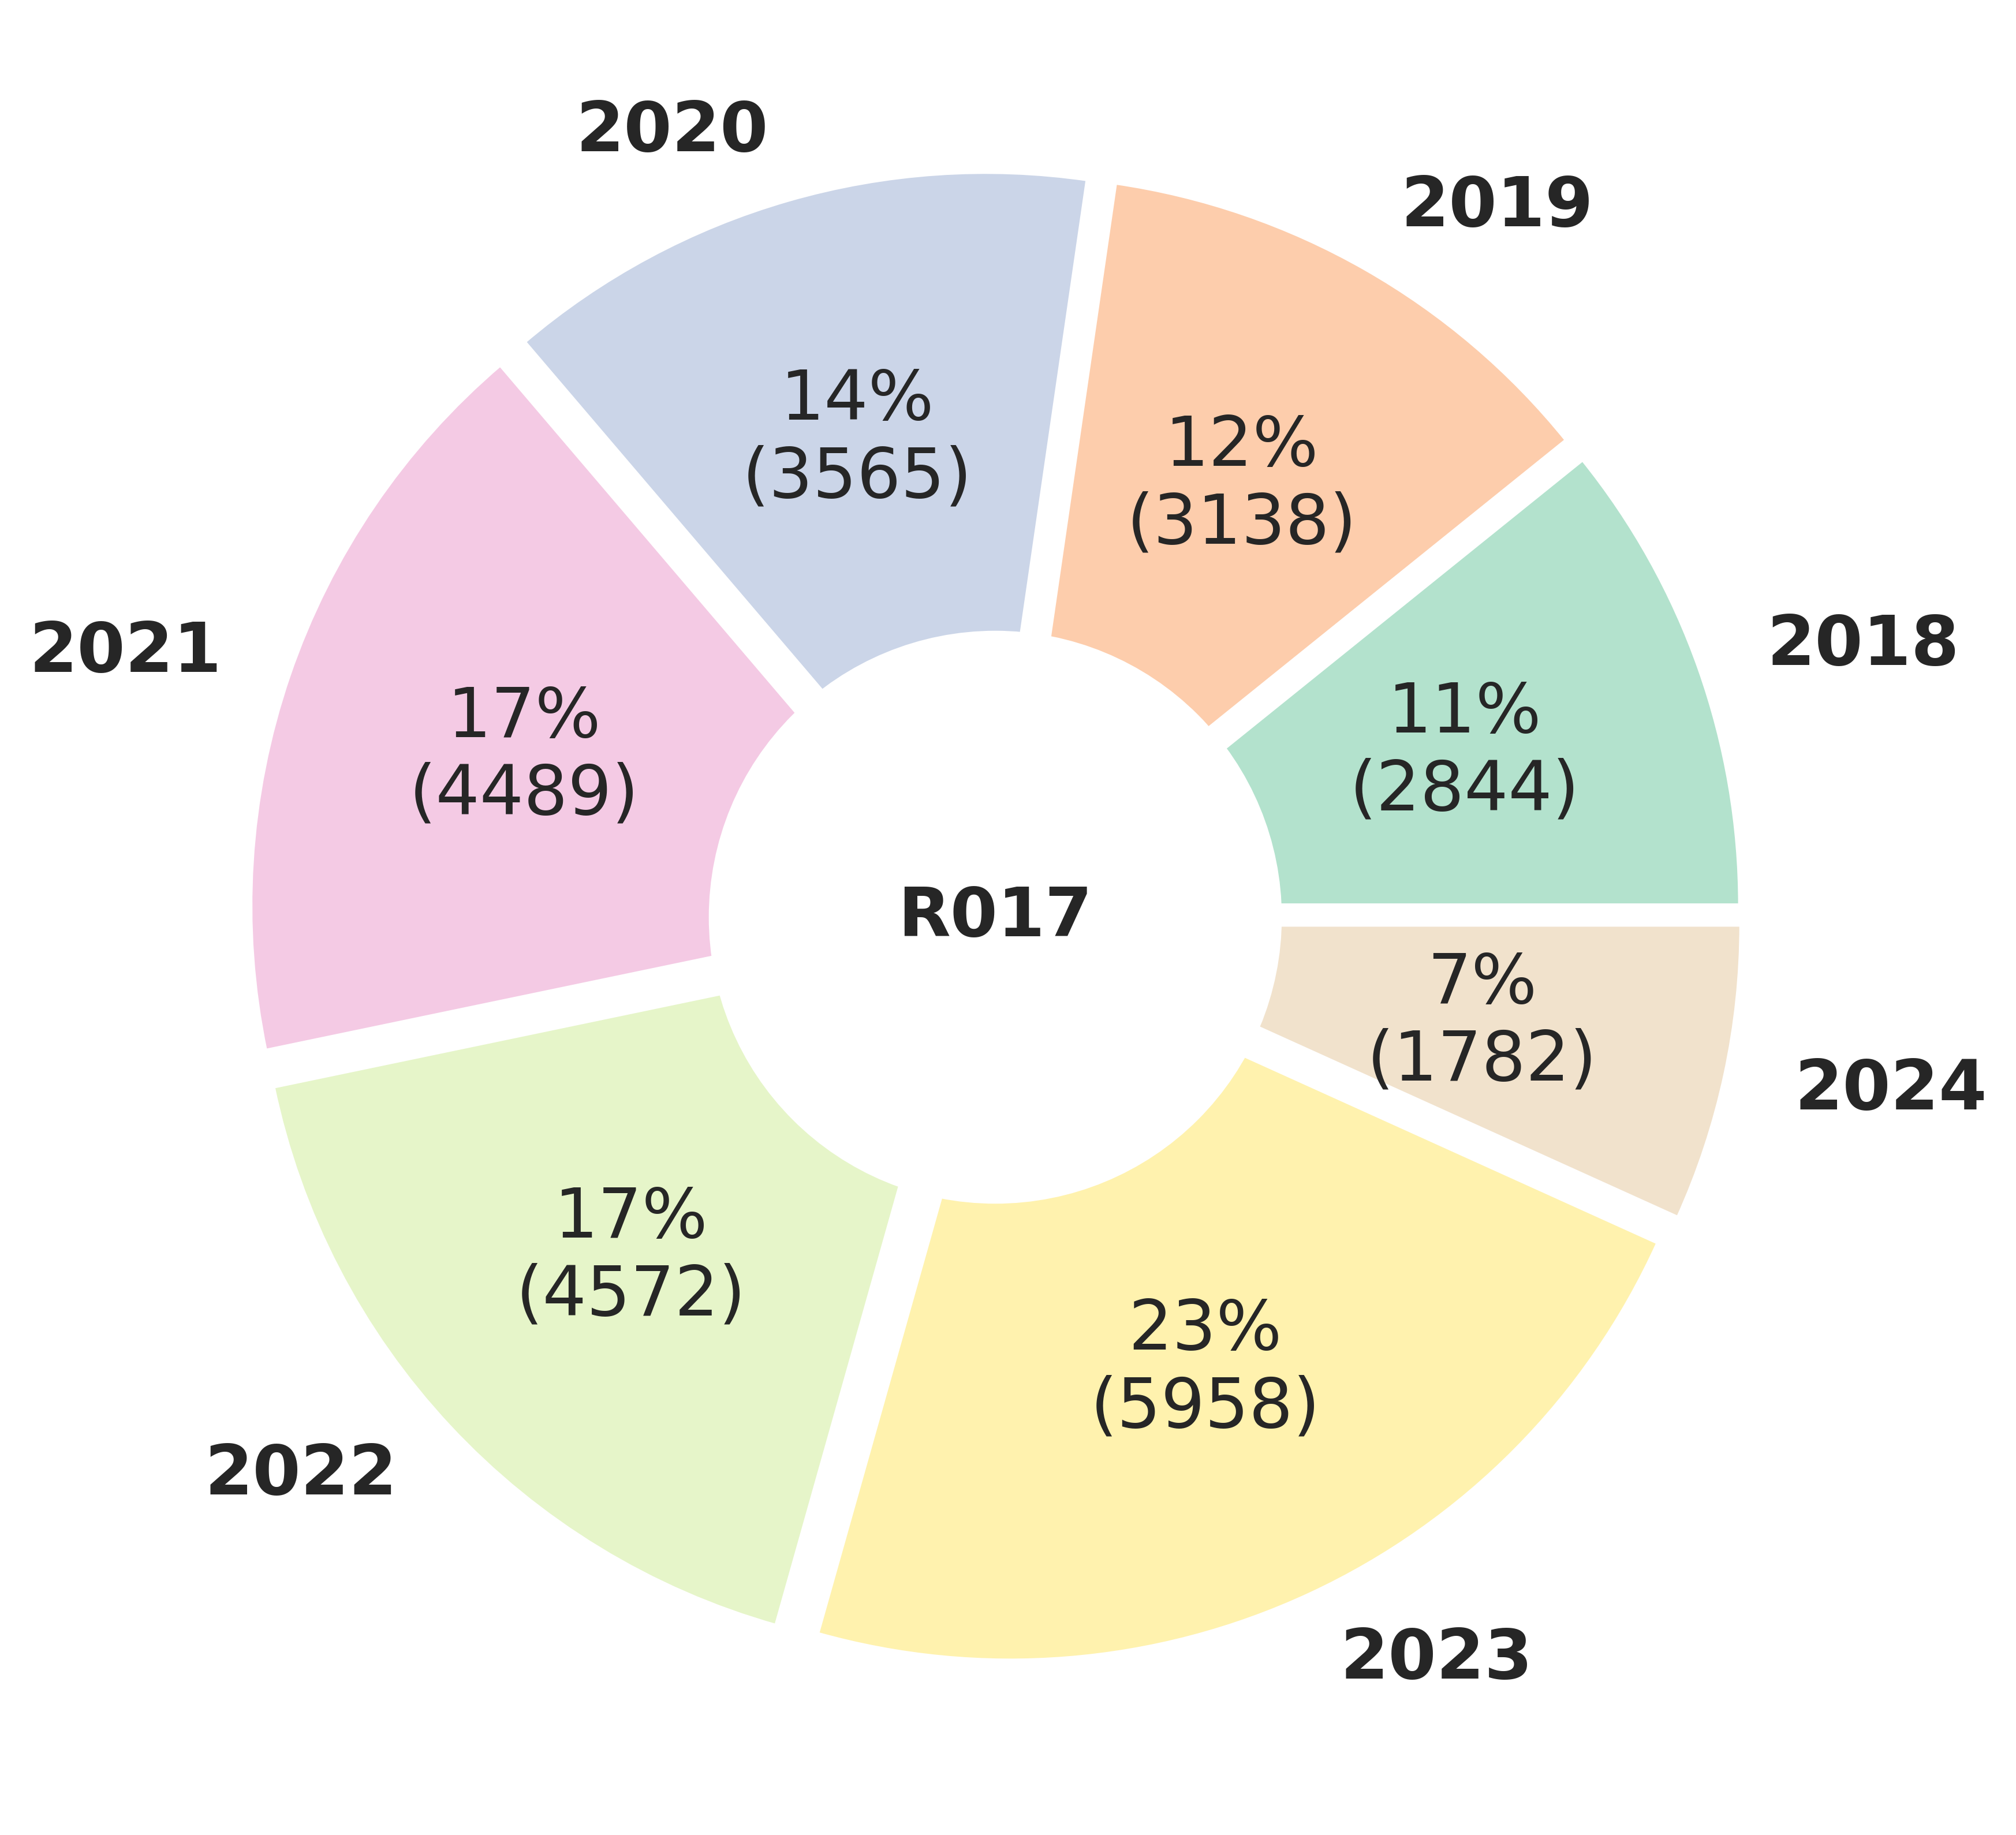
\includegraphics[width=\linewidth]{imagens/final/circle_R017.png}
		\caption{Número de contratos sinalizados para o indicador R017, por ano.}
		\label{final3}
		
	\end{minipage}
\end{figure}




\begin{figure}[H]
	\centering
	\begin{minipage}{.44\linewidth}
		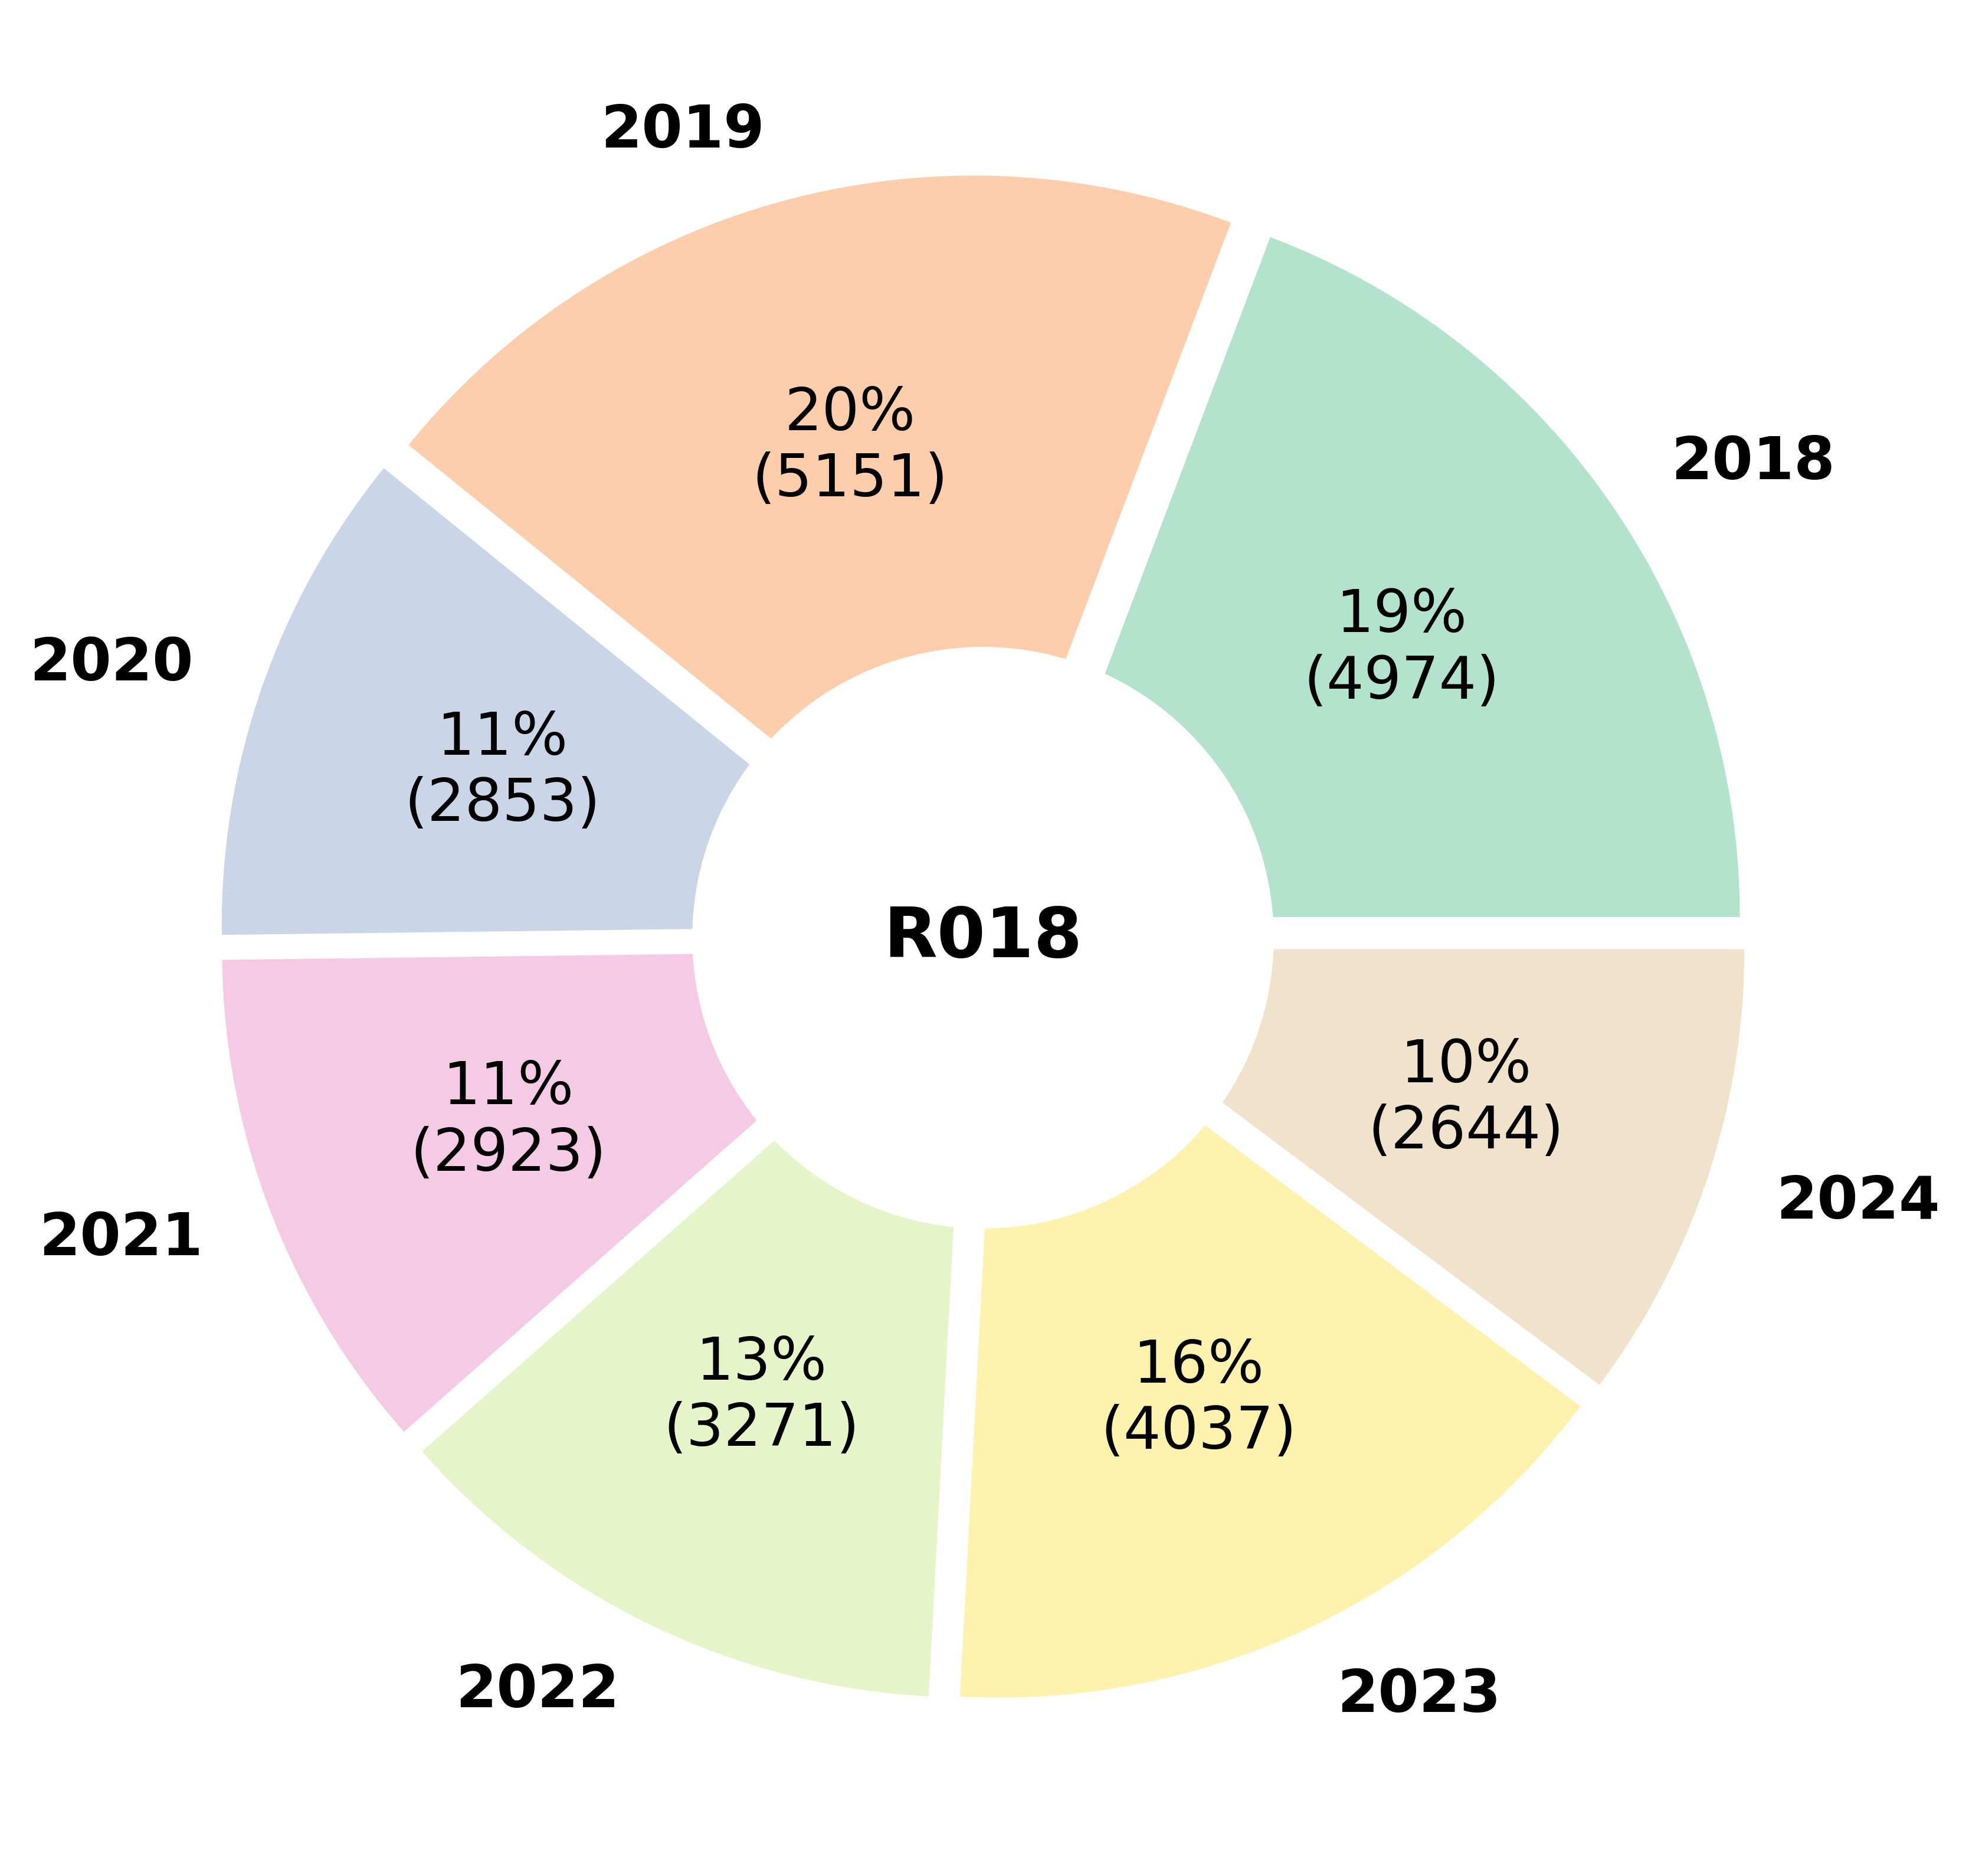
\includegraphics[width=\linewidth]{imagens/final/circle_R018.png}
		\caption{Número de contratos sinalizados para o indicador R018, por ano.}
		\label{final4}
		
	\end{minipage}
	\hfill
	\begin{minipage}{.44\linewidth}
		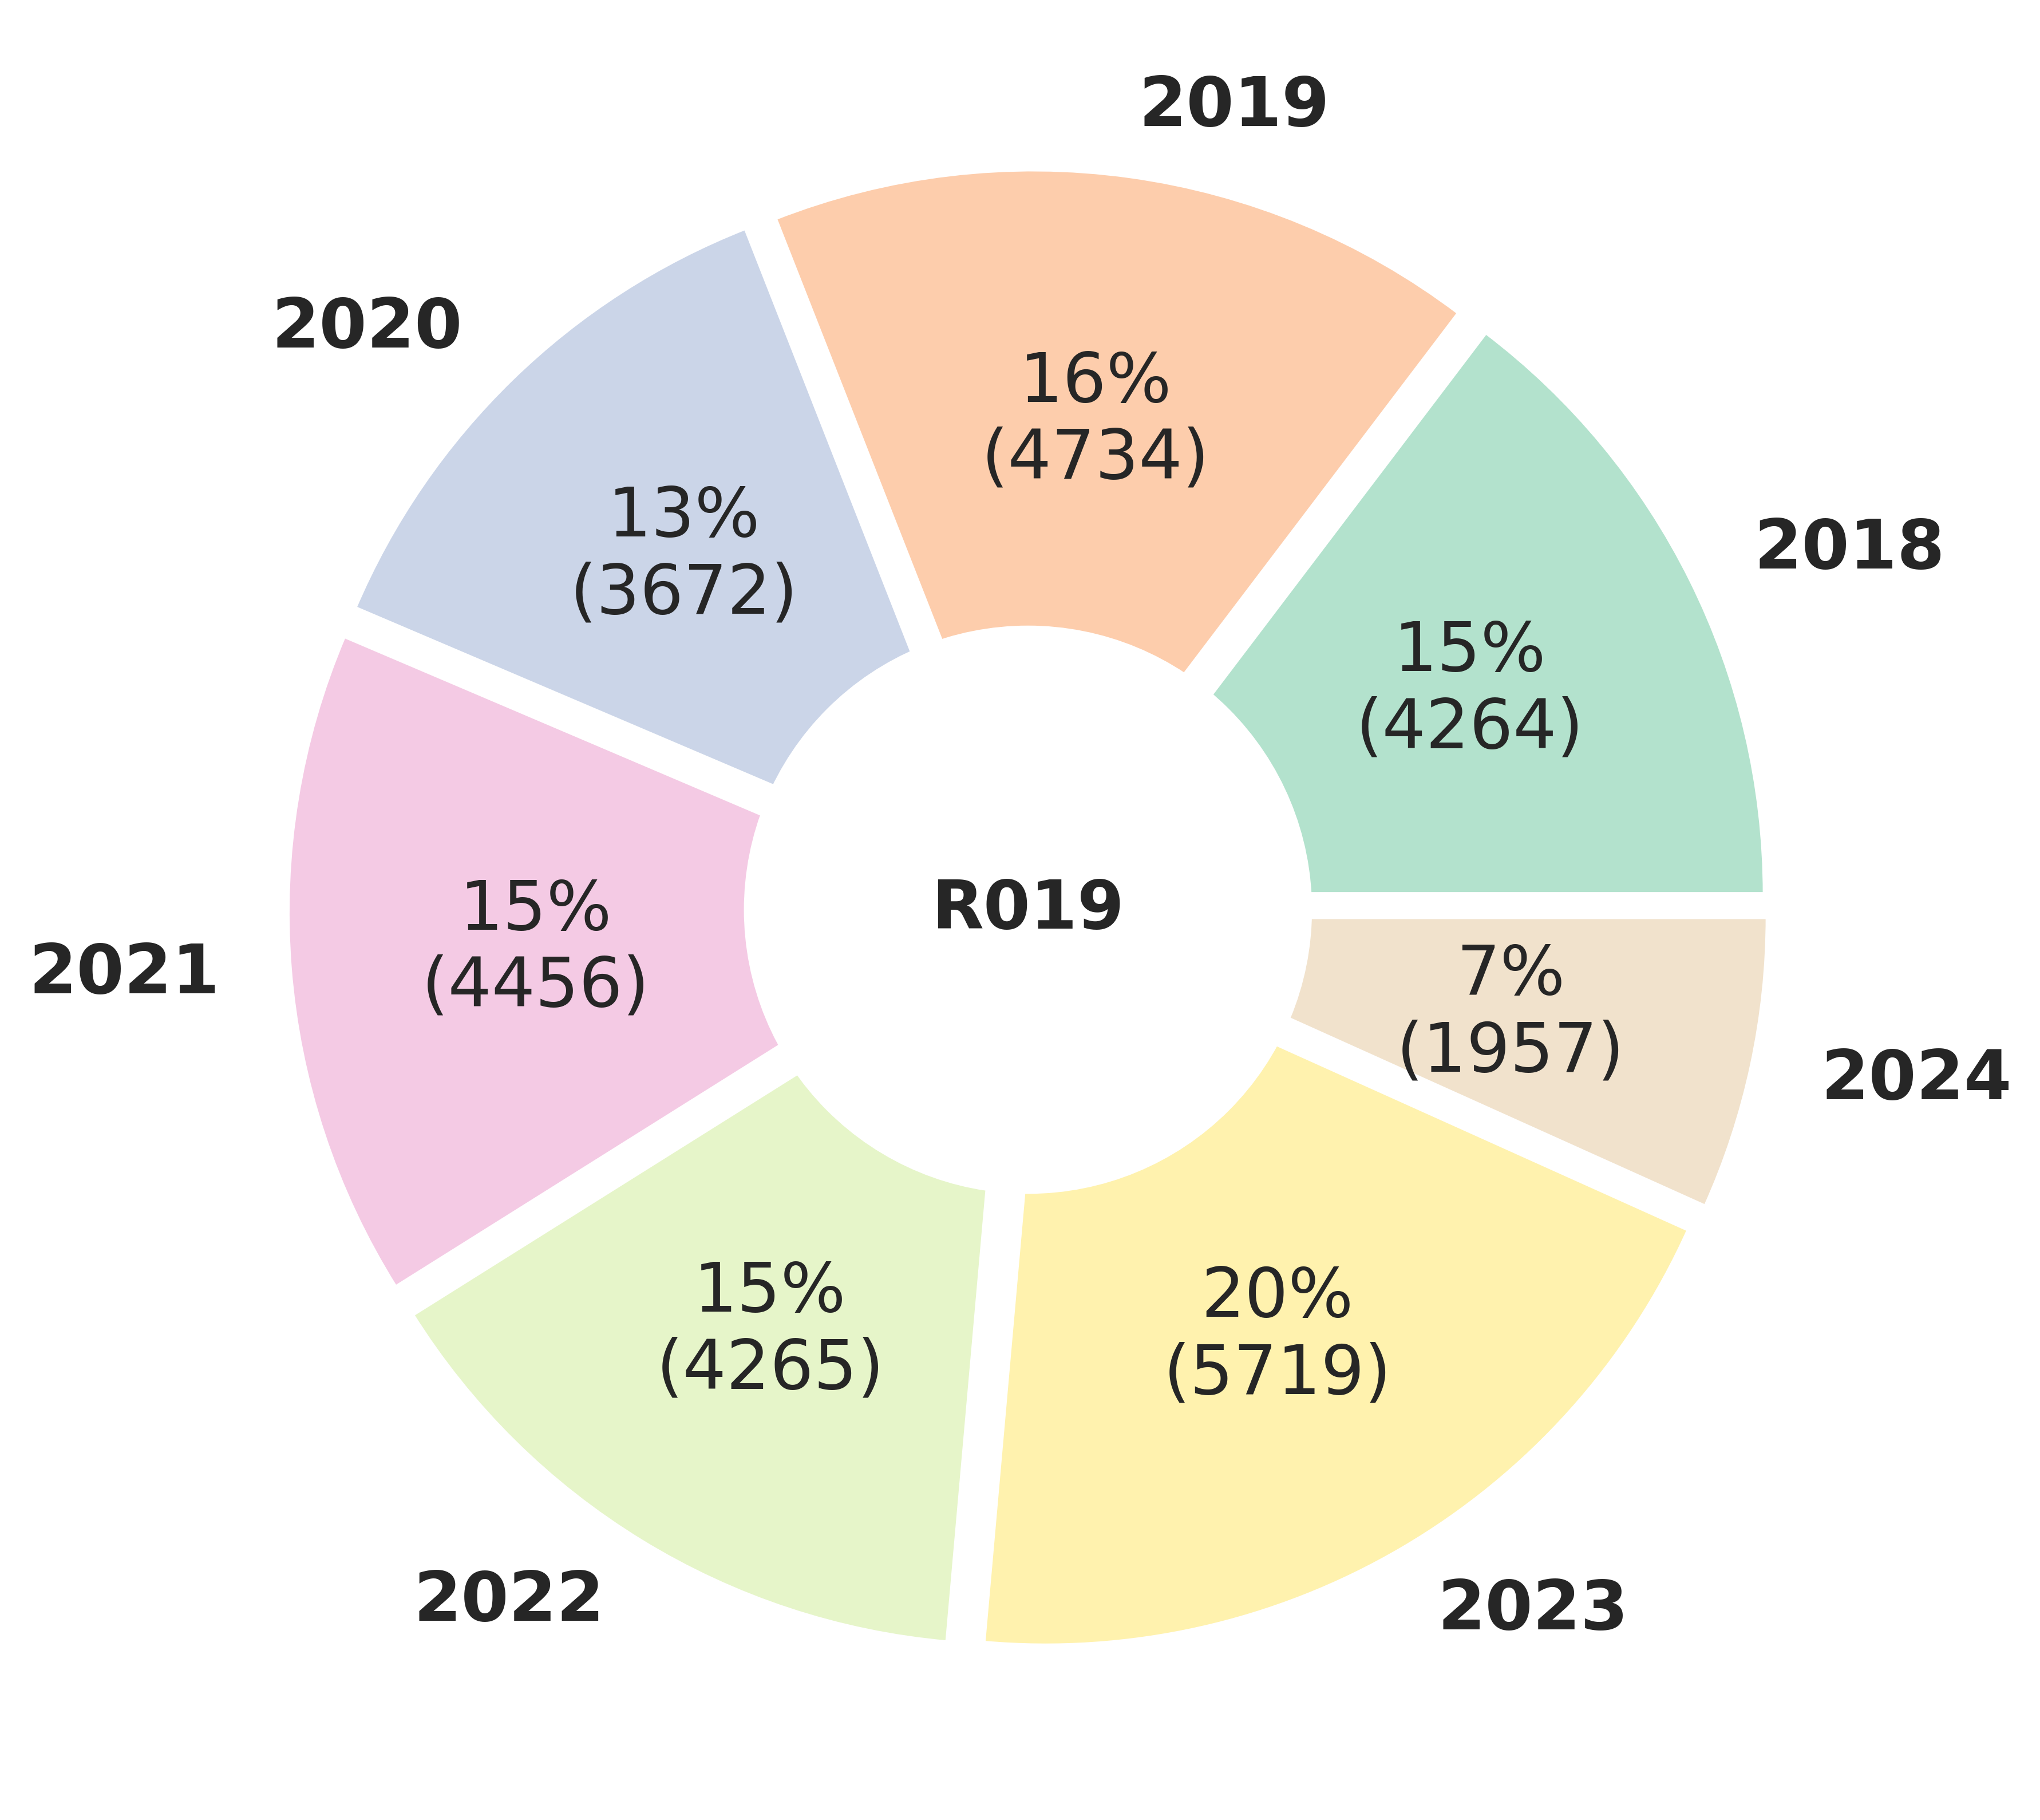
\includegraphics[width=\linewidth]{imagens/final/circle_R019.png}
		\caption{Número de contratos sinalizados para o indicador R019, por ano.}
		\label{final5}
				
	\end{minipage}
\end{figure}




\begin{figure}[H]
	\centering
	\begin{minipage}{.44\linewidth}
		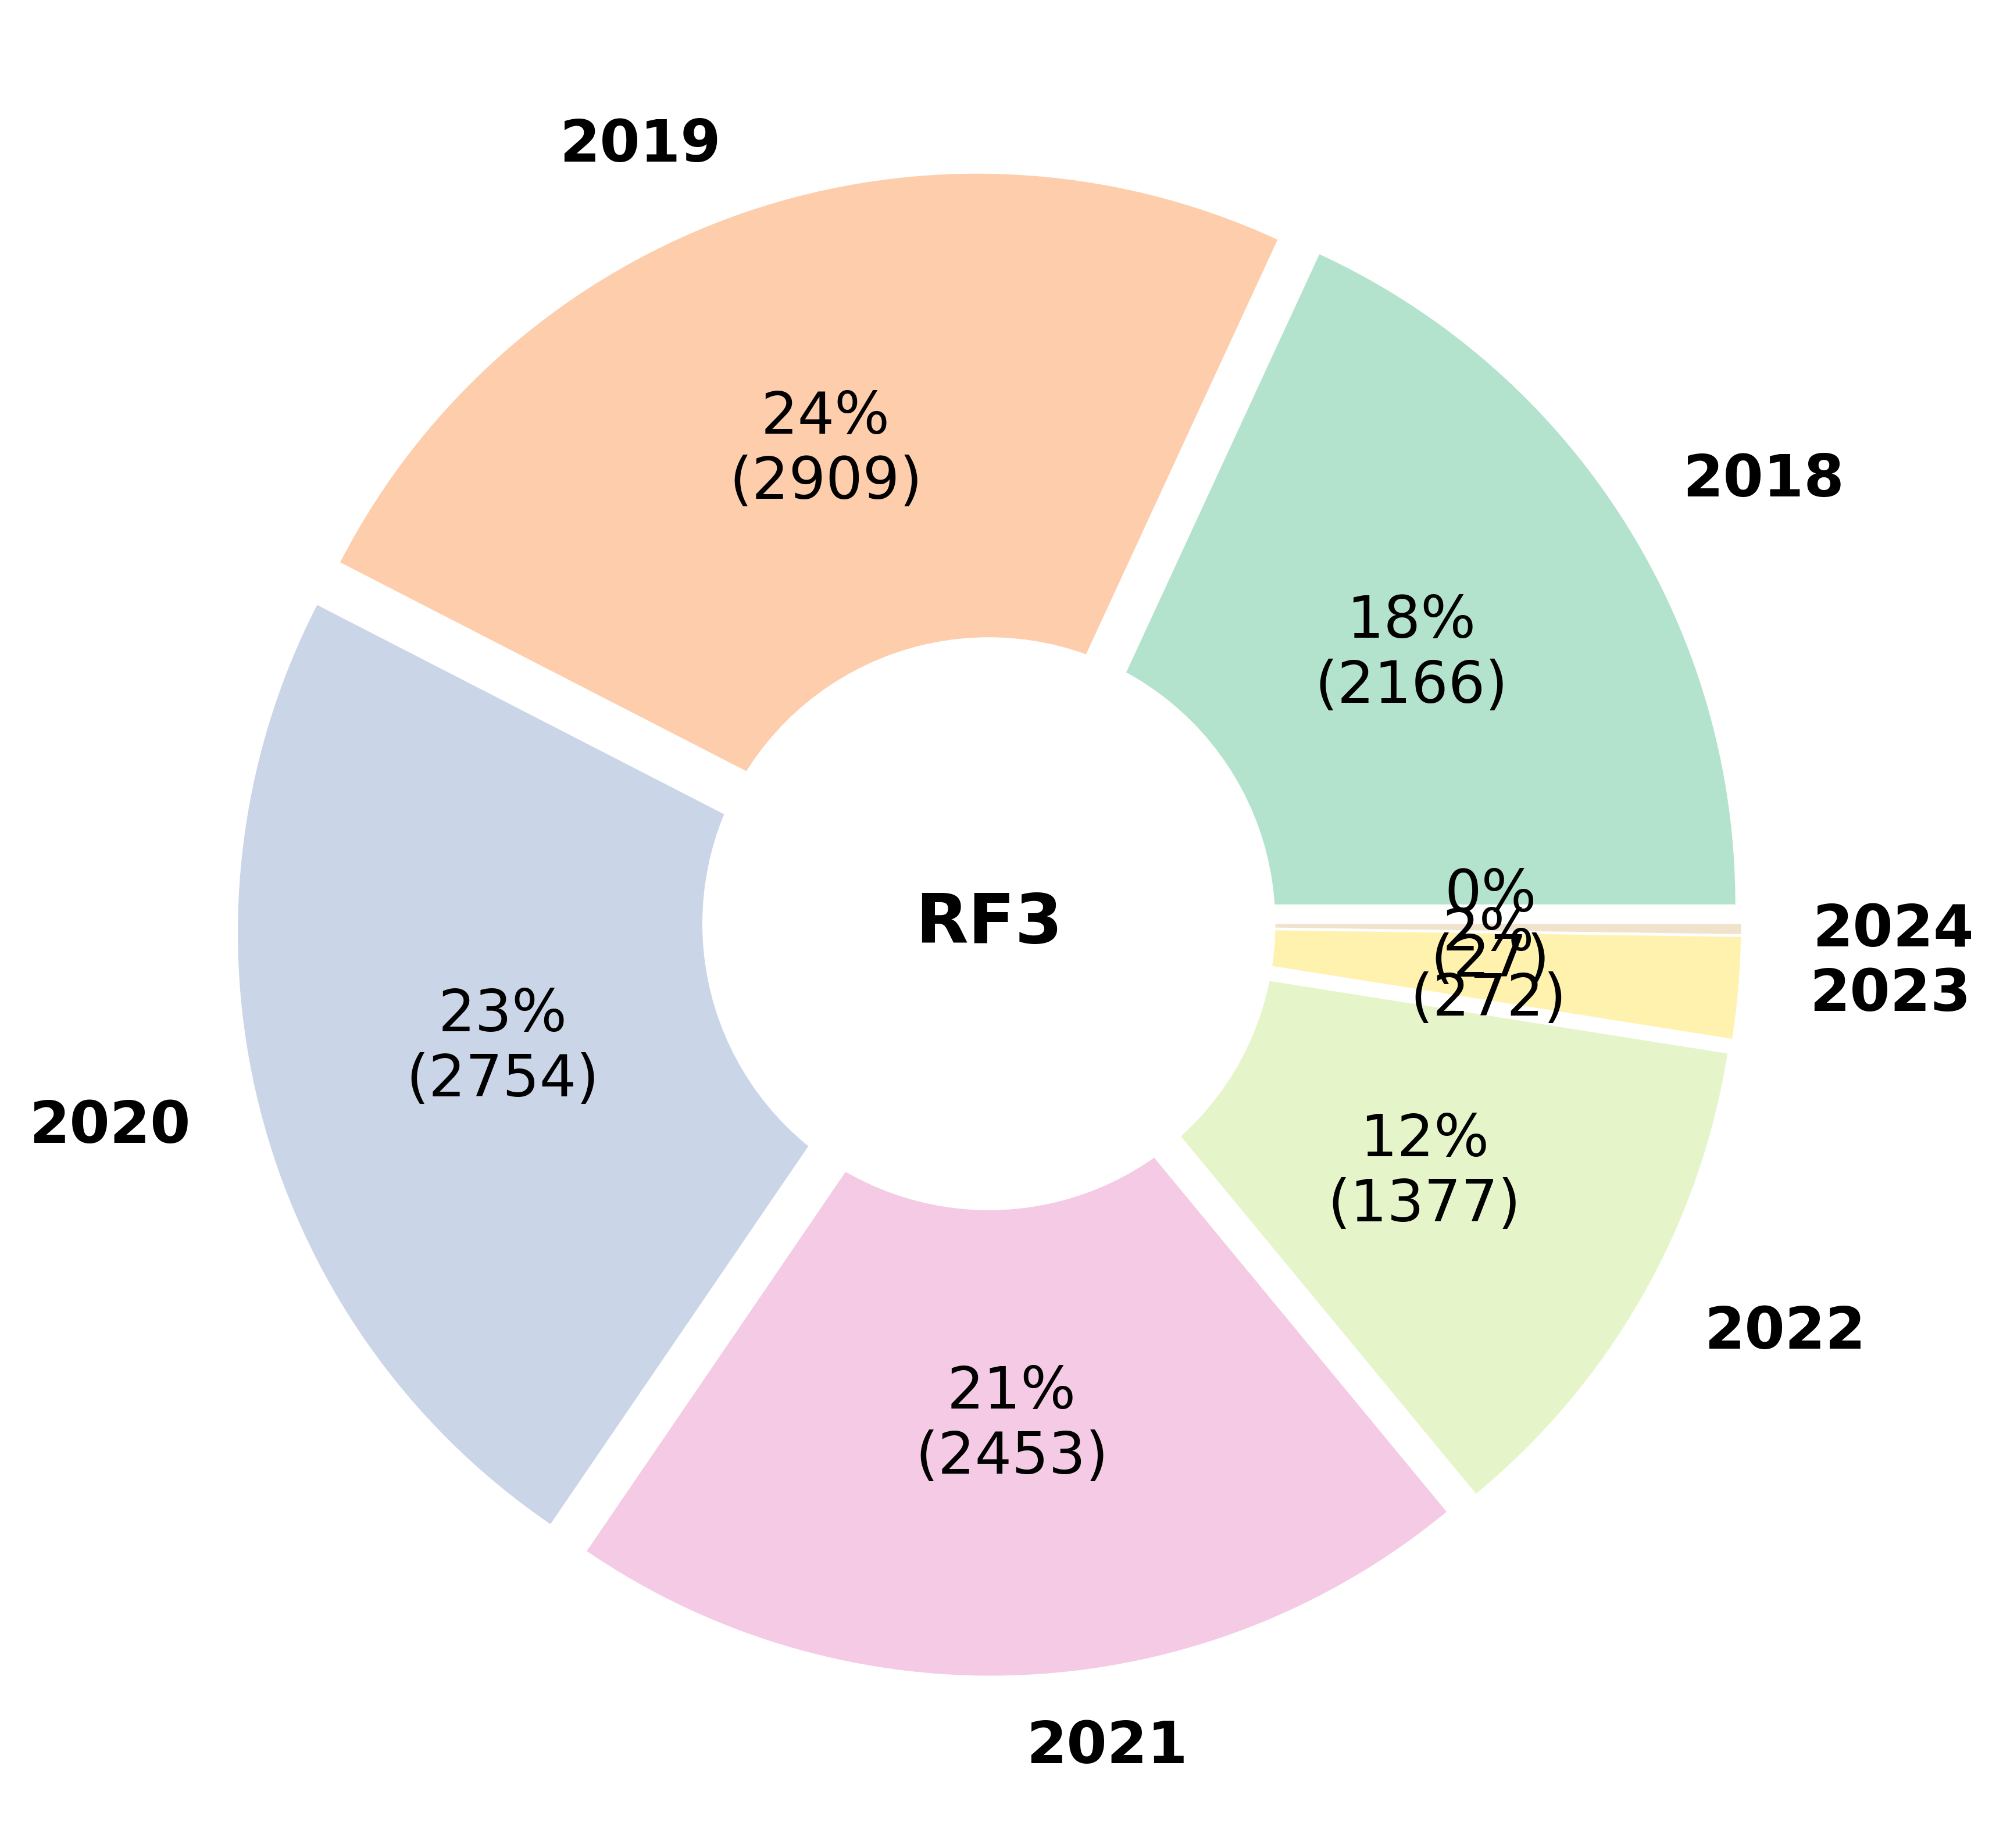
\includegraphics[width=\linewidth]{imagens/final/circle_RF3.png}
		\caption{Número de contratos sinalizados para o indicador RF3, por ano.}
		\label{final6}
		
	\end{minipage}
	\hfill
	\begin{minipage}{.44\linewidth}
		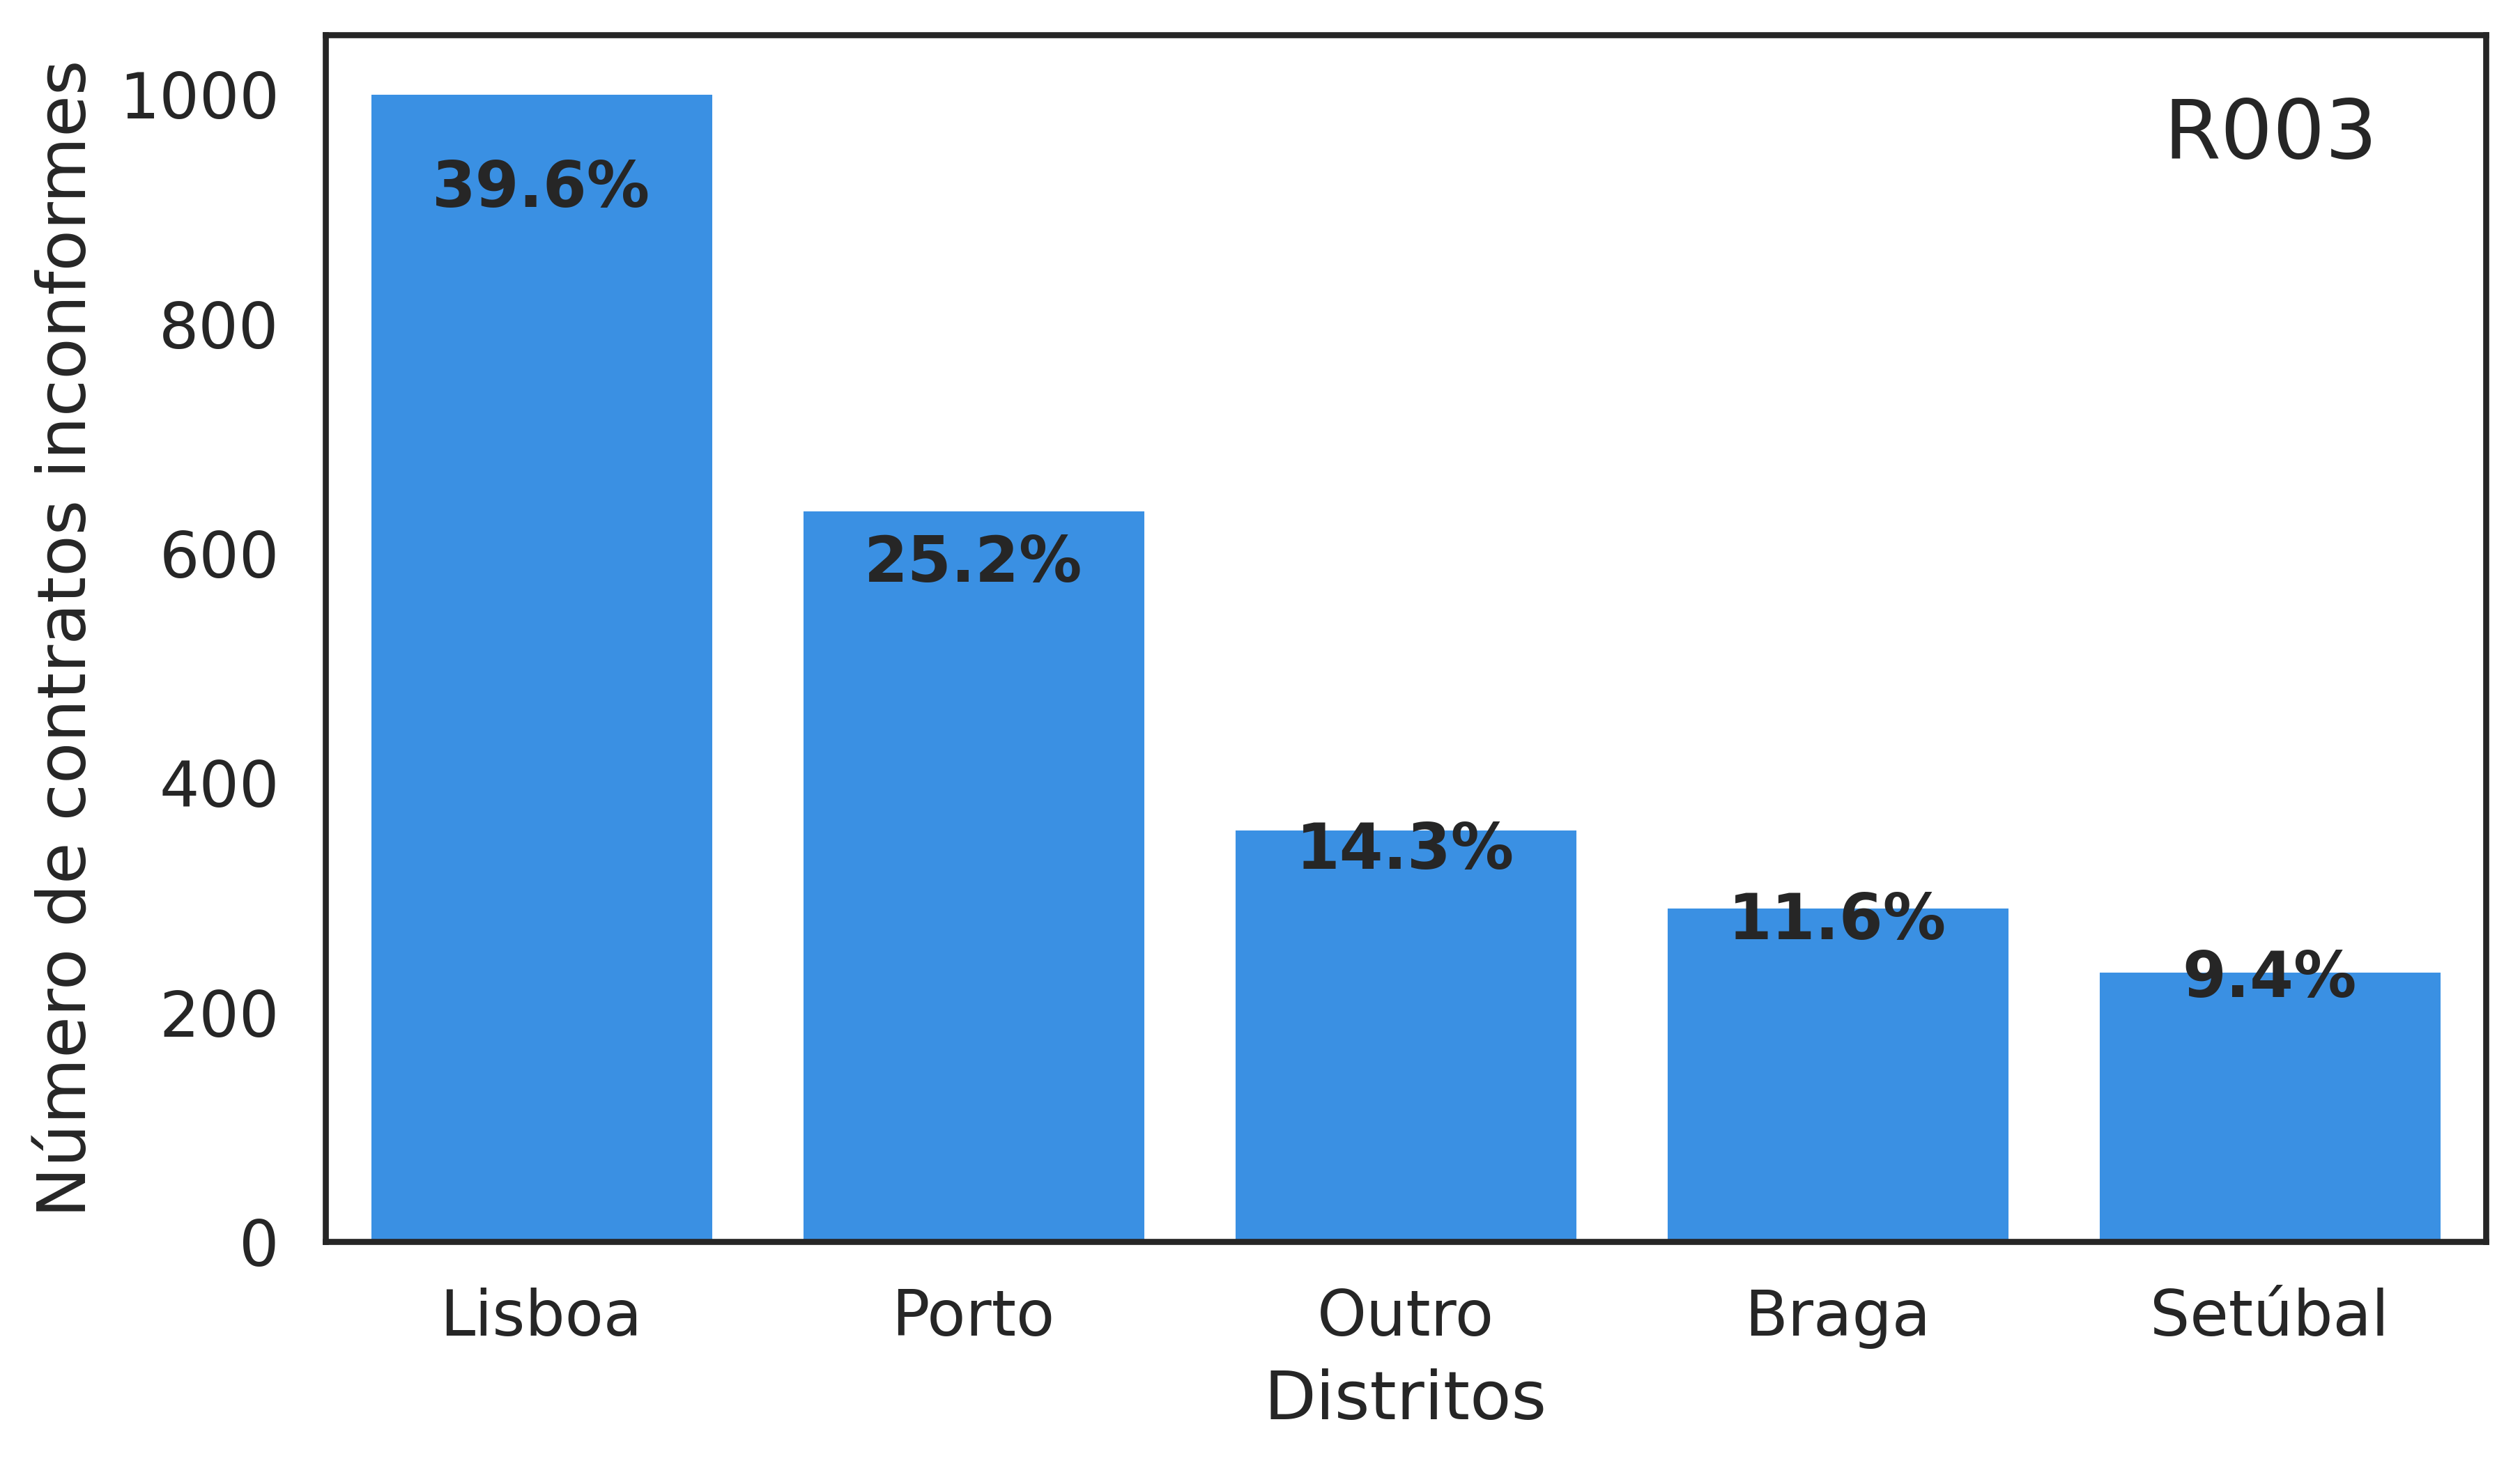
\includegraphics[width=\linewidth]{imagens/final/bar_R003.png}
		\caption{Número de contratos sinalizados para o indicador R003, por distrito.}
		\label{final7}
		
	\end{minipage}
\end{figure}


As Figuras \ref{final7}, \ref{final8}, \ref{final9}, \ref{final10} e \ref{final11} são elucidativas da forma como se distribuem, para cada flag, o número absoluto, e respetiva percentagem, de contratos sinalizados, por distrito. Concordante com a Figura \ref{fig:distritos}, o distrito com maior percentagem de contratos sinalizados, transversal a todas as flags, é Lisboa. Existe uma percentagem significativa de distritos caracterizados como \textit{Outro}, o que, de certa forma, deturpa os valores apresentados. Se preenchidos os distritos de forma correta, verificar-se-ia um número de contratos sinalizados ainda maior, possivelmente, para os já apresentados. Na zona norte destacam-se os distritos do Porto e Braga, enquanto que na zona sul o foco recai nos distritos de Setúbal e Faro. 



\begin{figure}[H]
	\centering
	\begin{minipage}{.44\linewidth}
		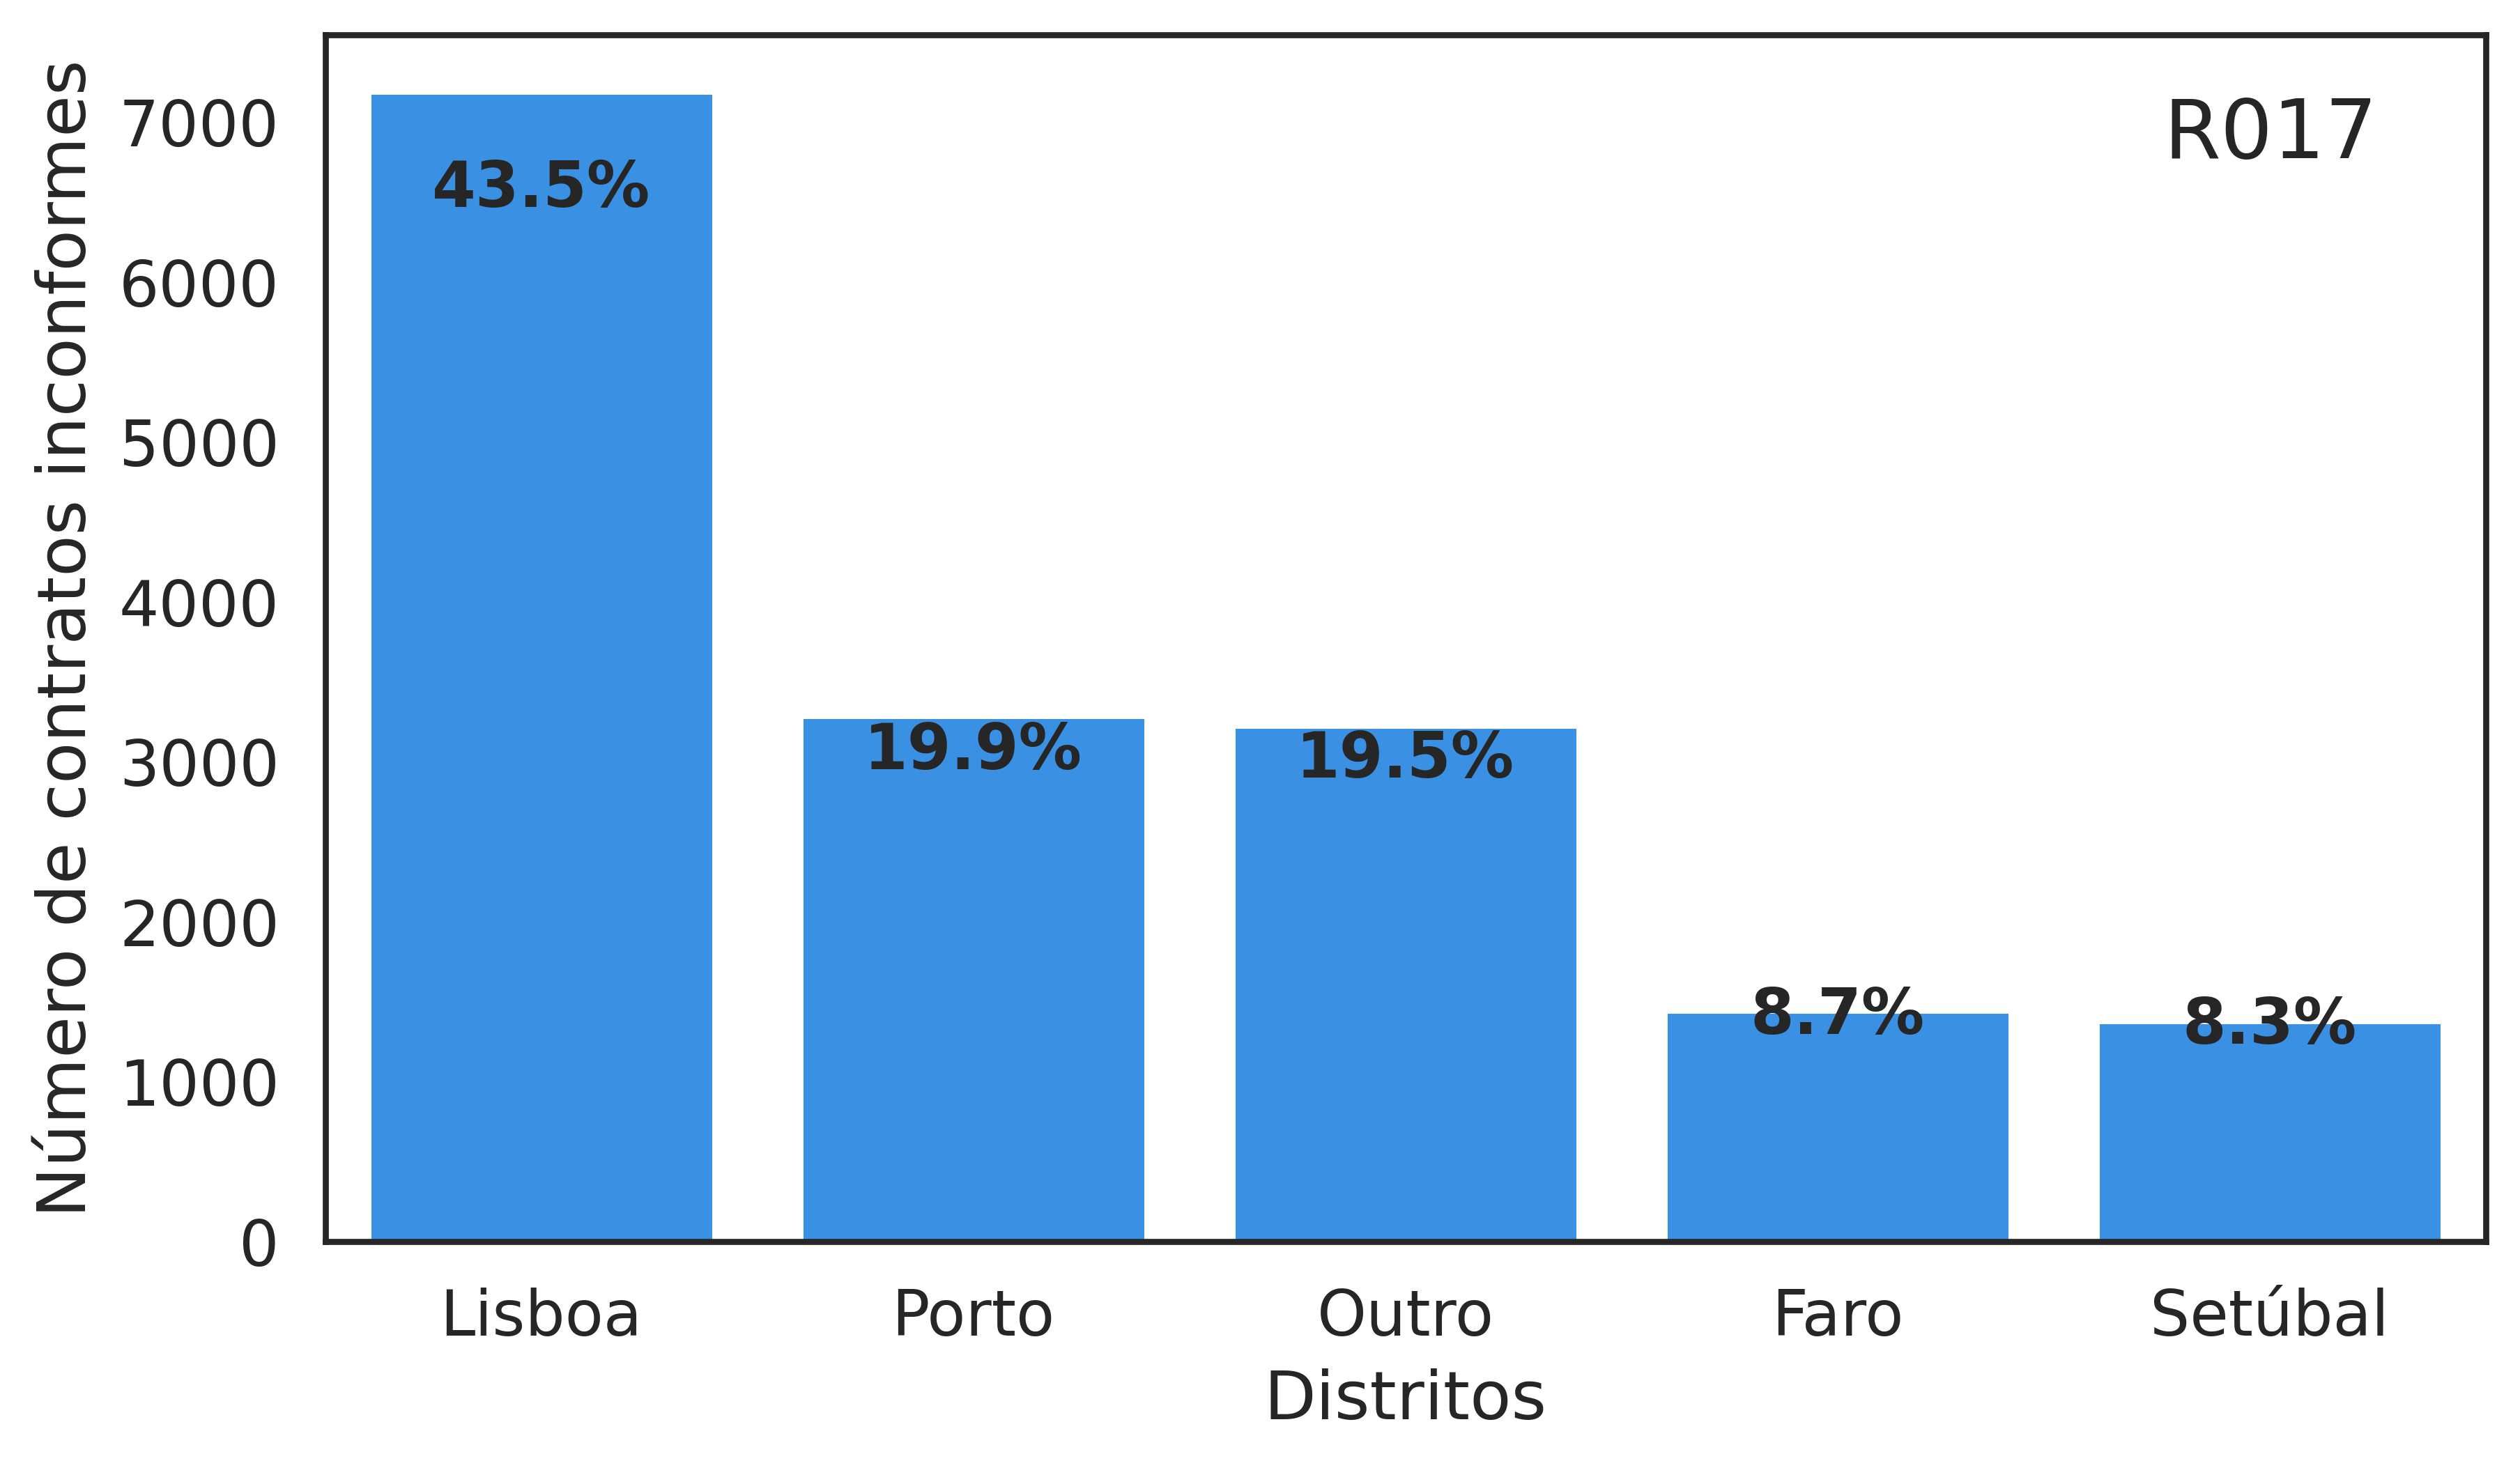
\includegraphics[width=\linewidth]{imagens/final/bar_R017.png}
				\caption{Número de contratos sinalizados para o indicador R017, por distrito.}
		\label{final8}
		
	\end{minipage}
	\hfill
	\begin{minipage}{.44\linewidth}
		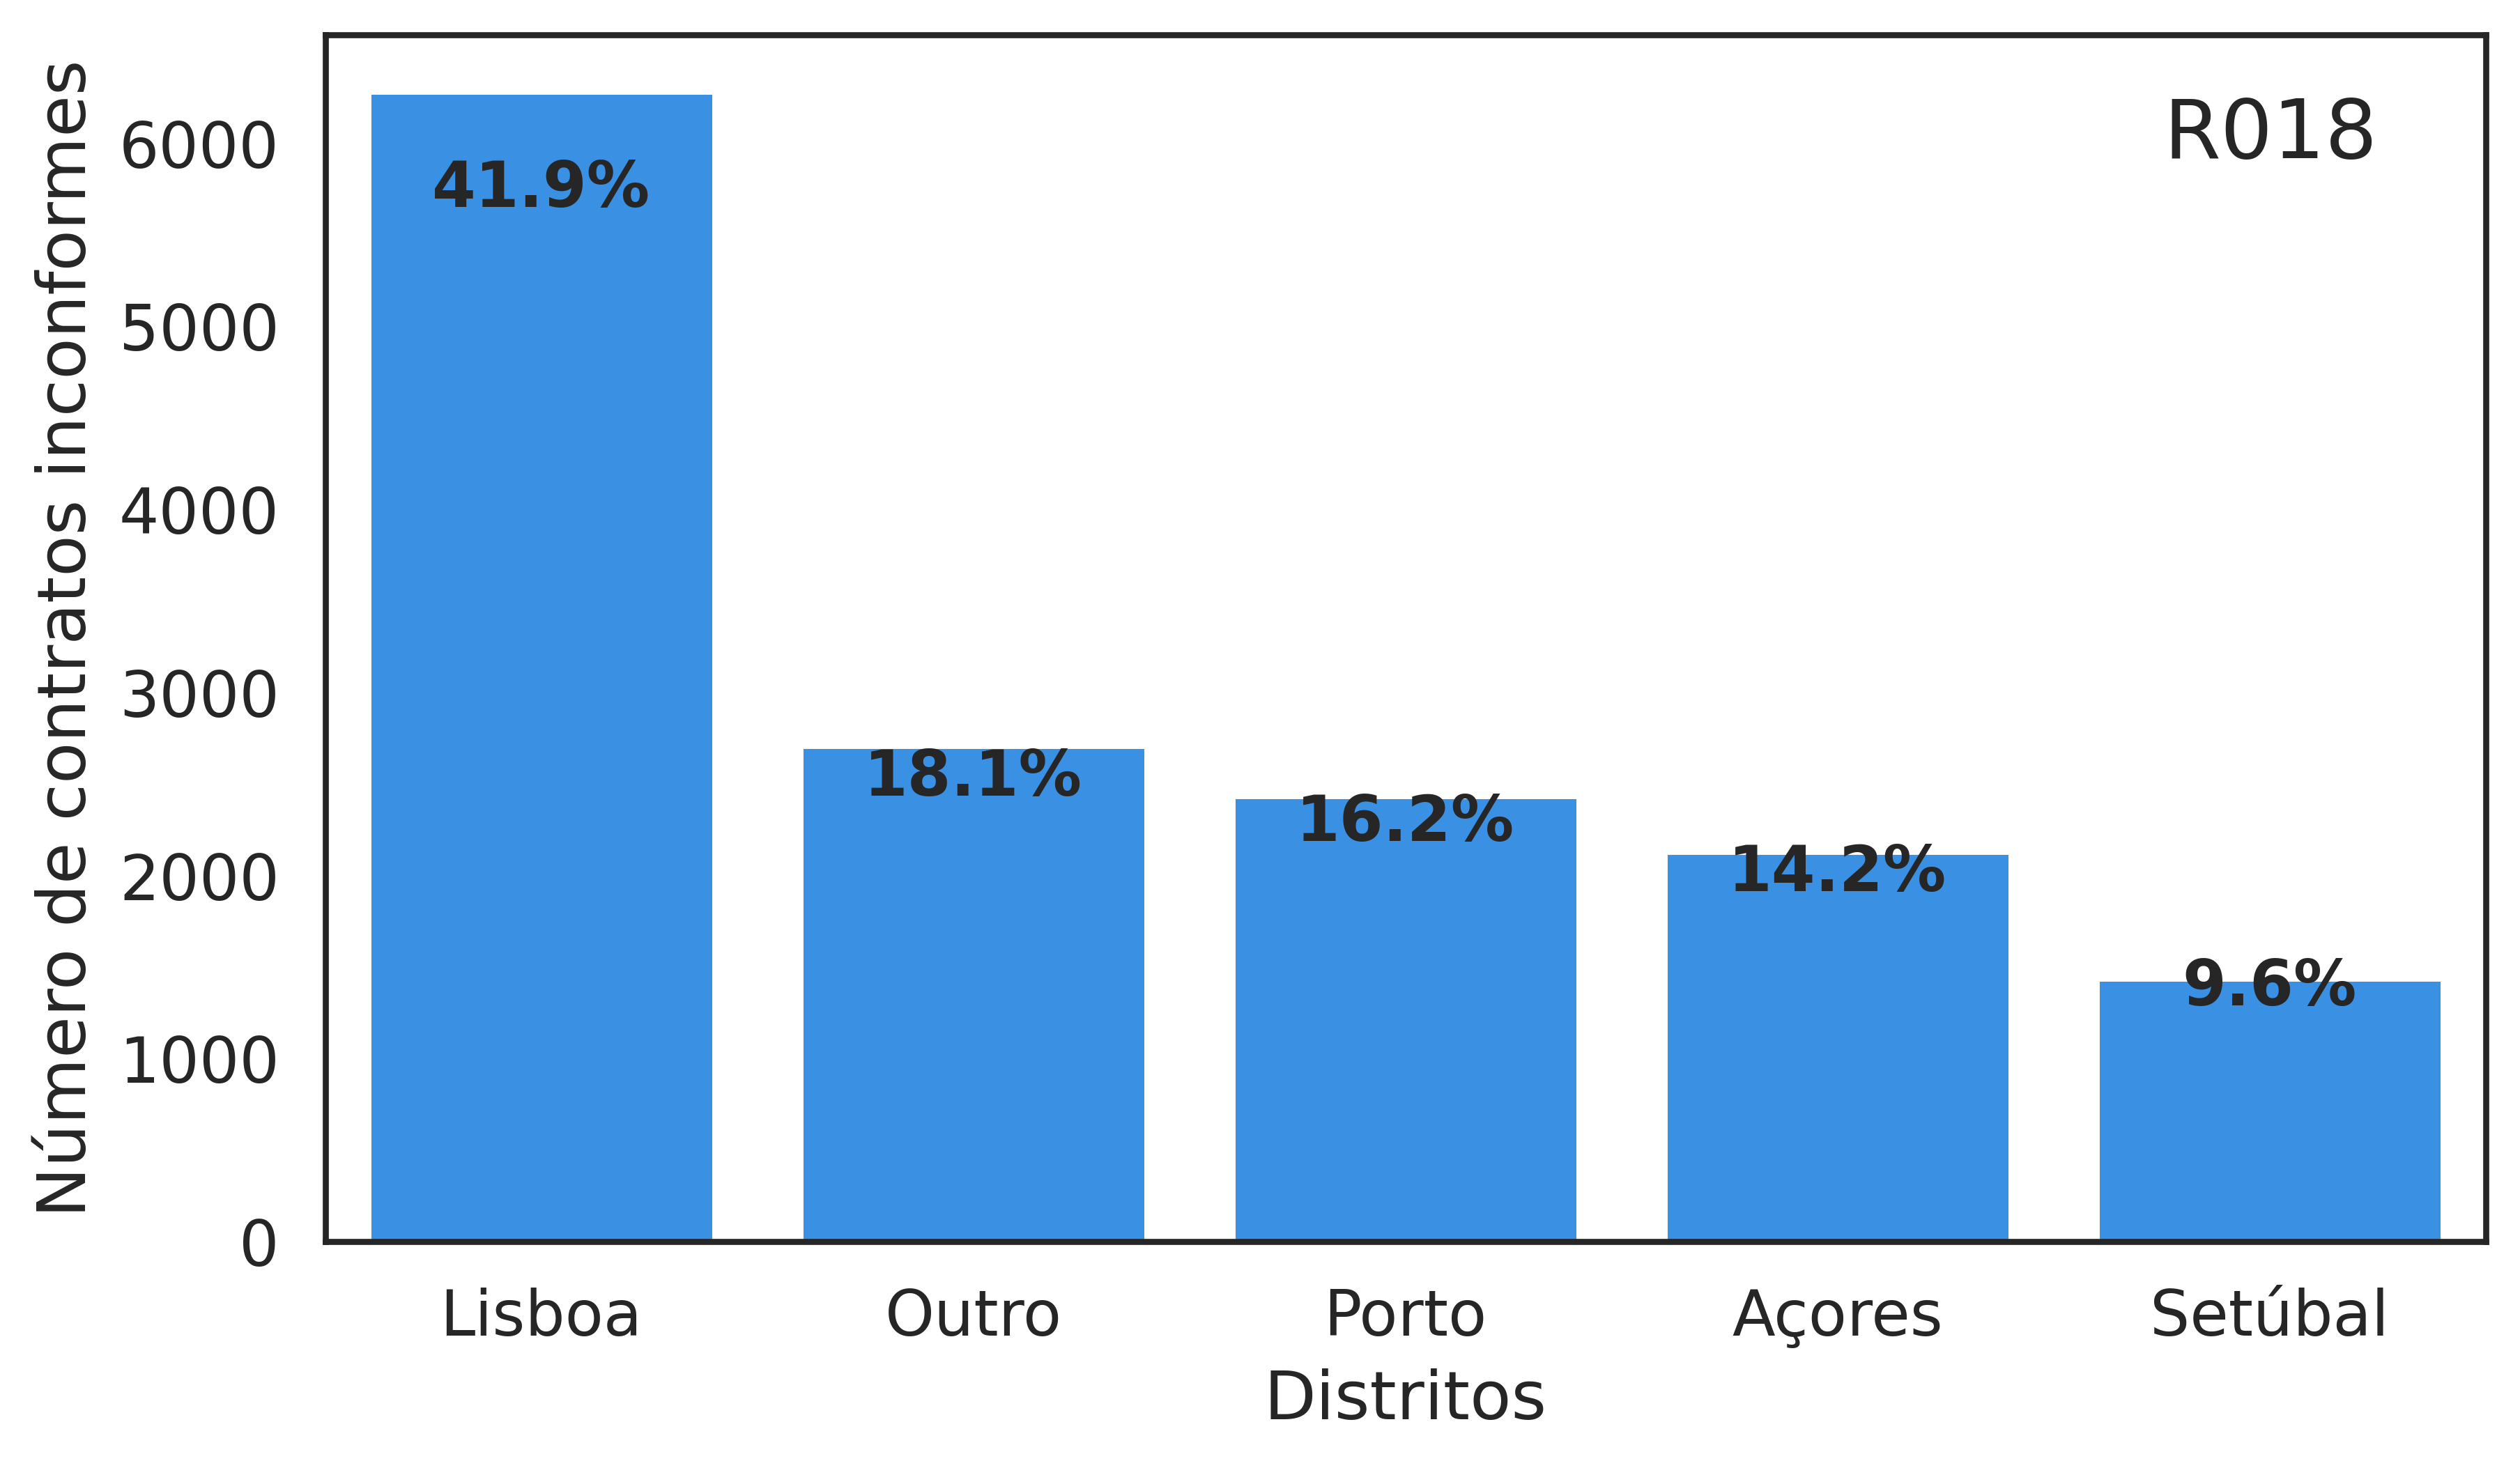
\includegraphics[width=\linewidth]{imagens/final/bar_R018.png}
		\caption{Número de contratos sinalizados para o indicador R018, por distrito.}
		\label{final9}
		
	\end{minipage}
\end{figure}


\begin{figure}[H]
	\centering
	\begin{minipage}{.44\linewidth}
		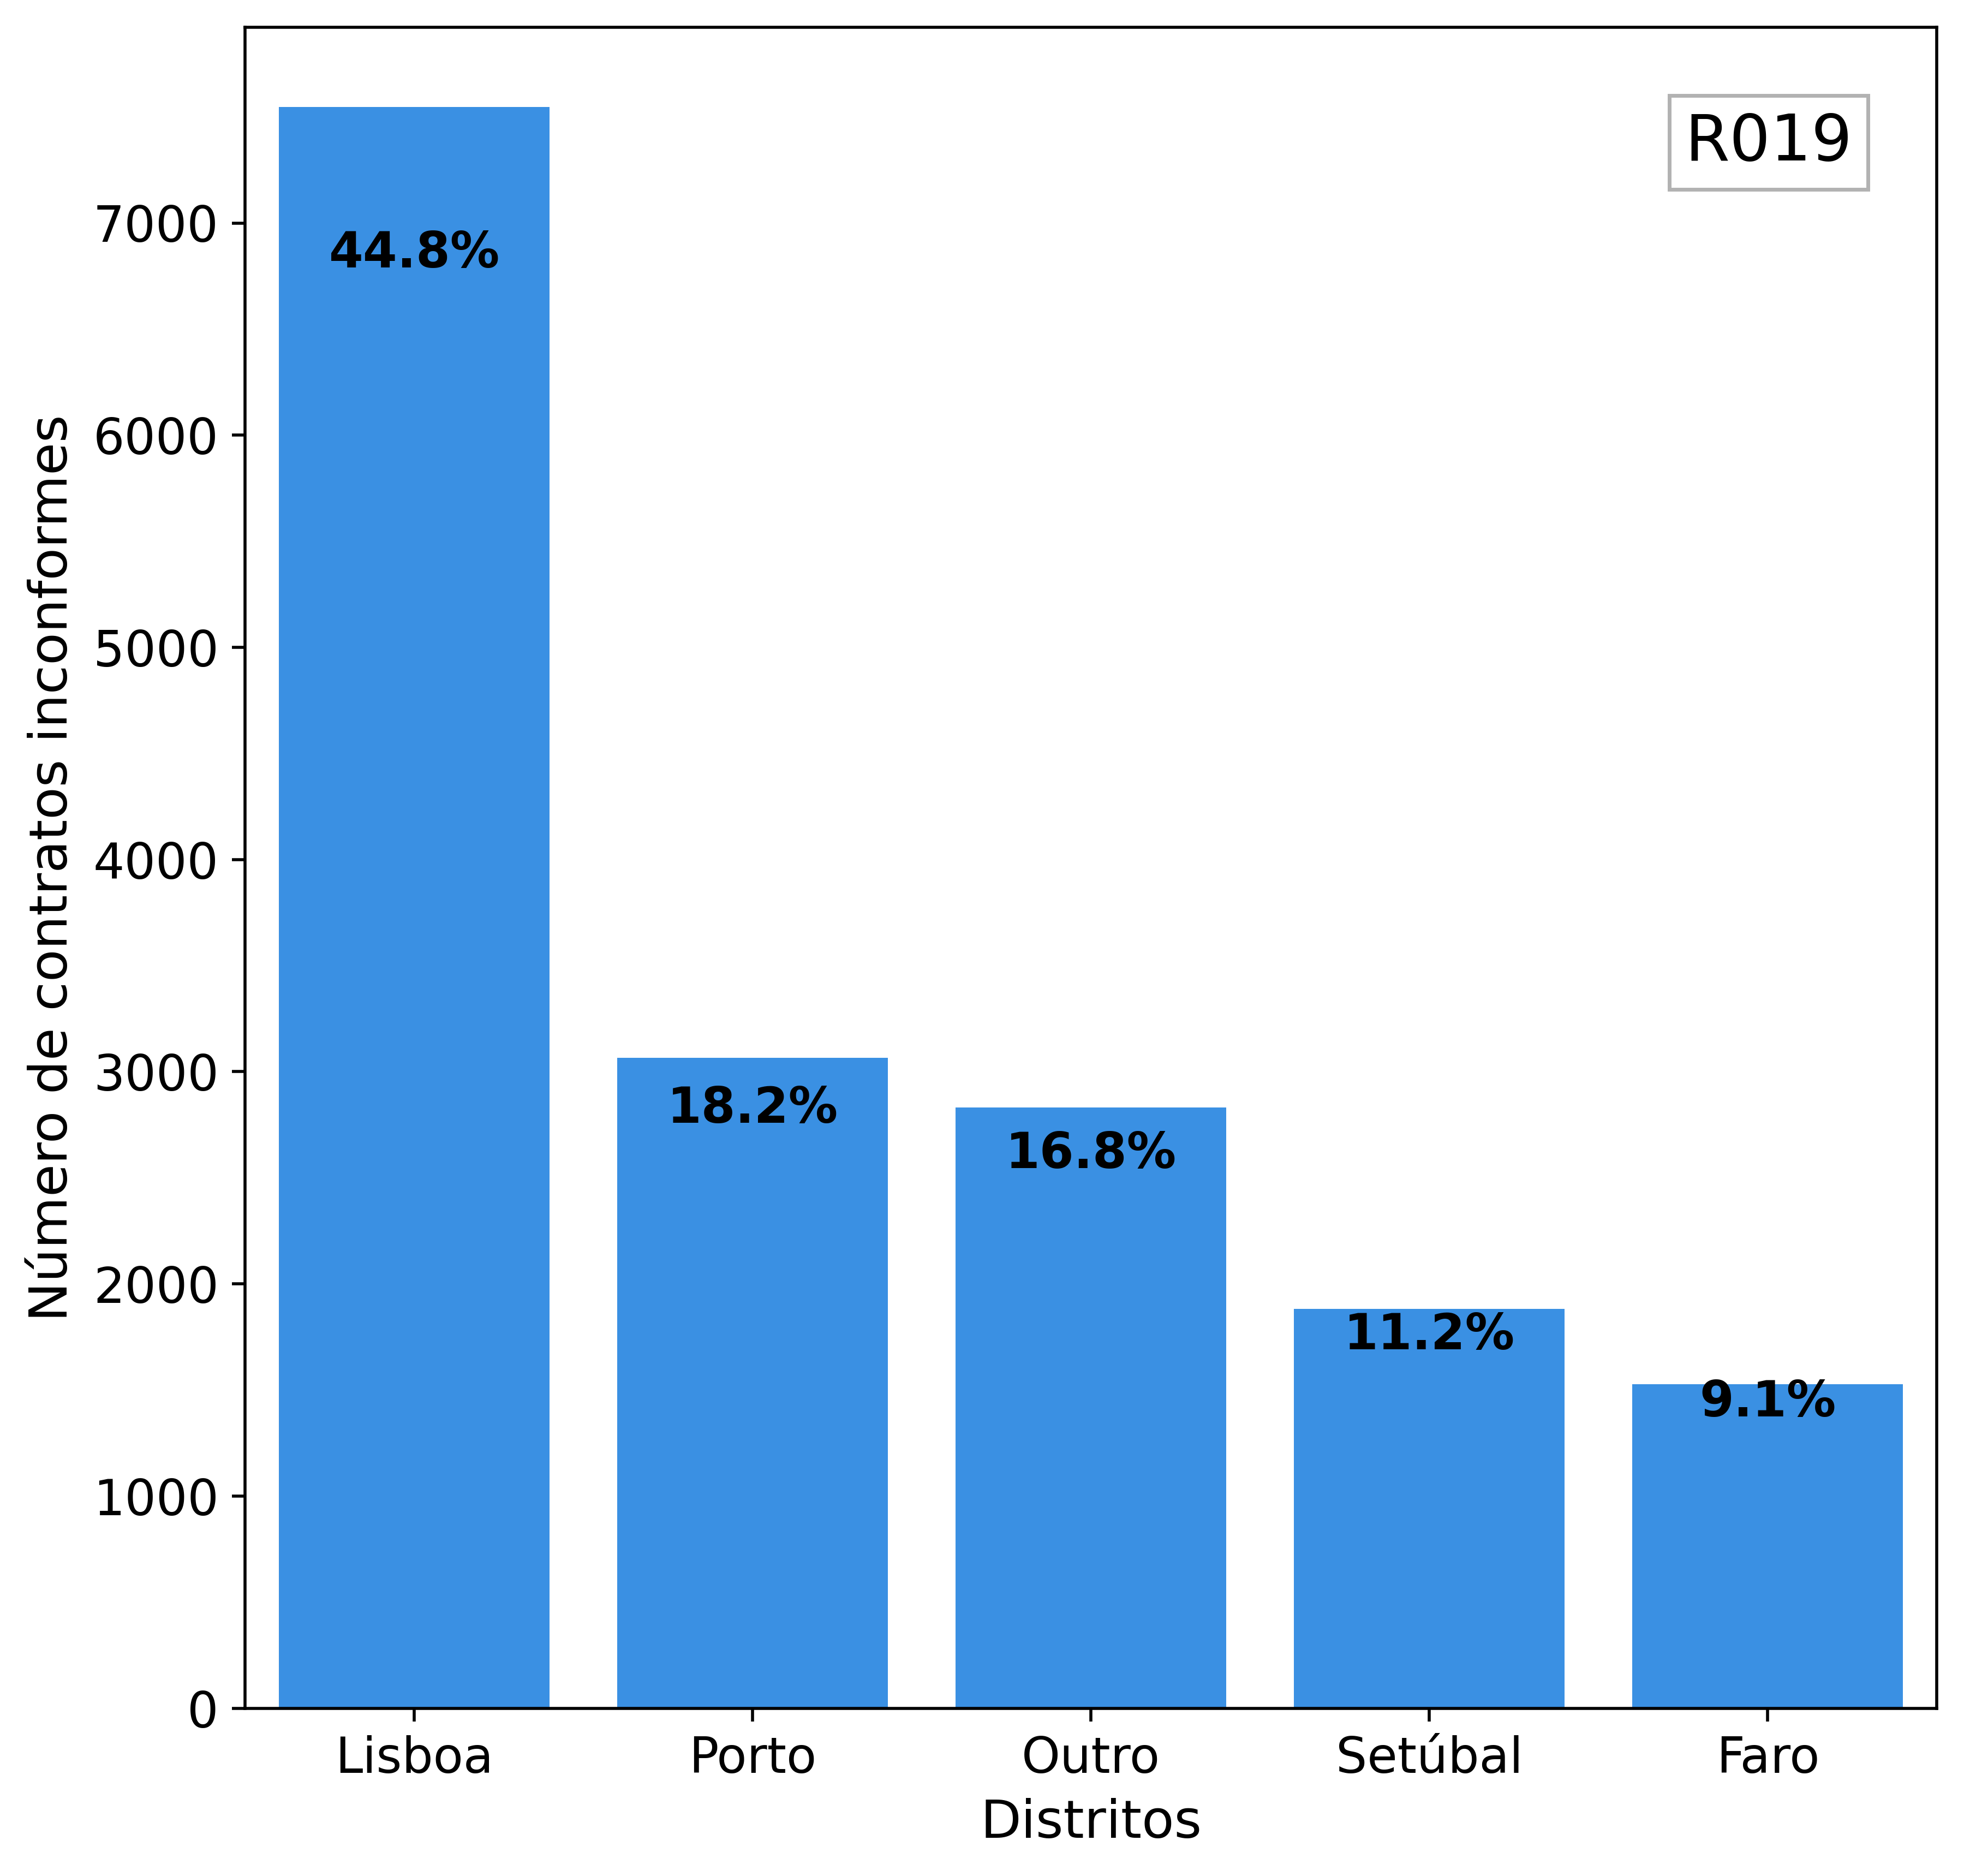
\includegraphics[width=\linewidth]{imagens/final/bar_R019.png}
		\caption{Número de contratos sinalizados para o indicador R019, por distrito.}
		\label{final10}
		
	\end{minipage}
	\hfill
	\begin{minipage}{.44\linewidth}
		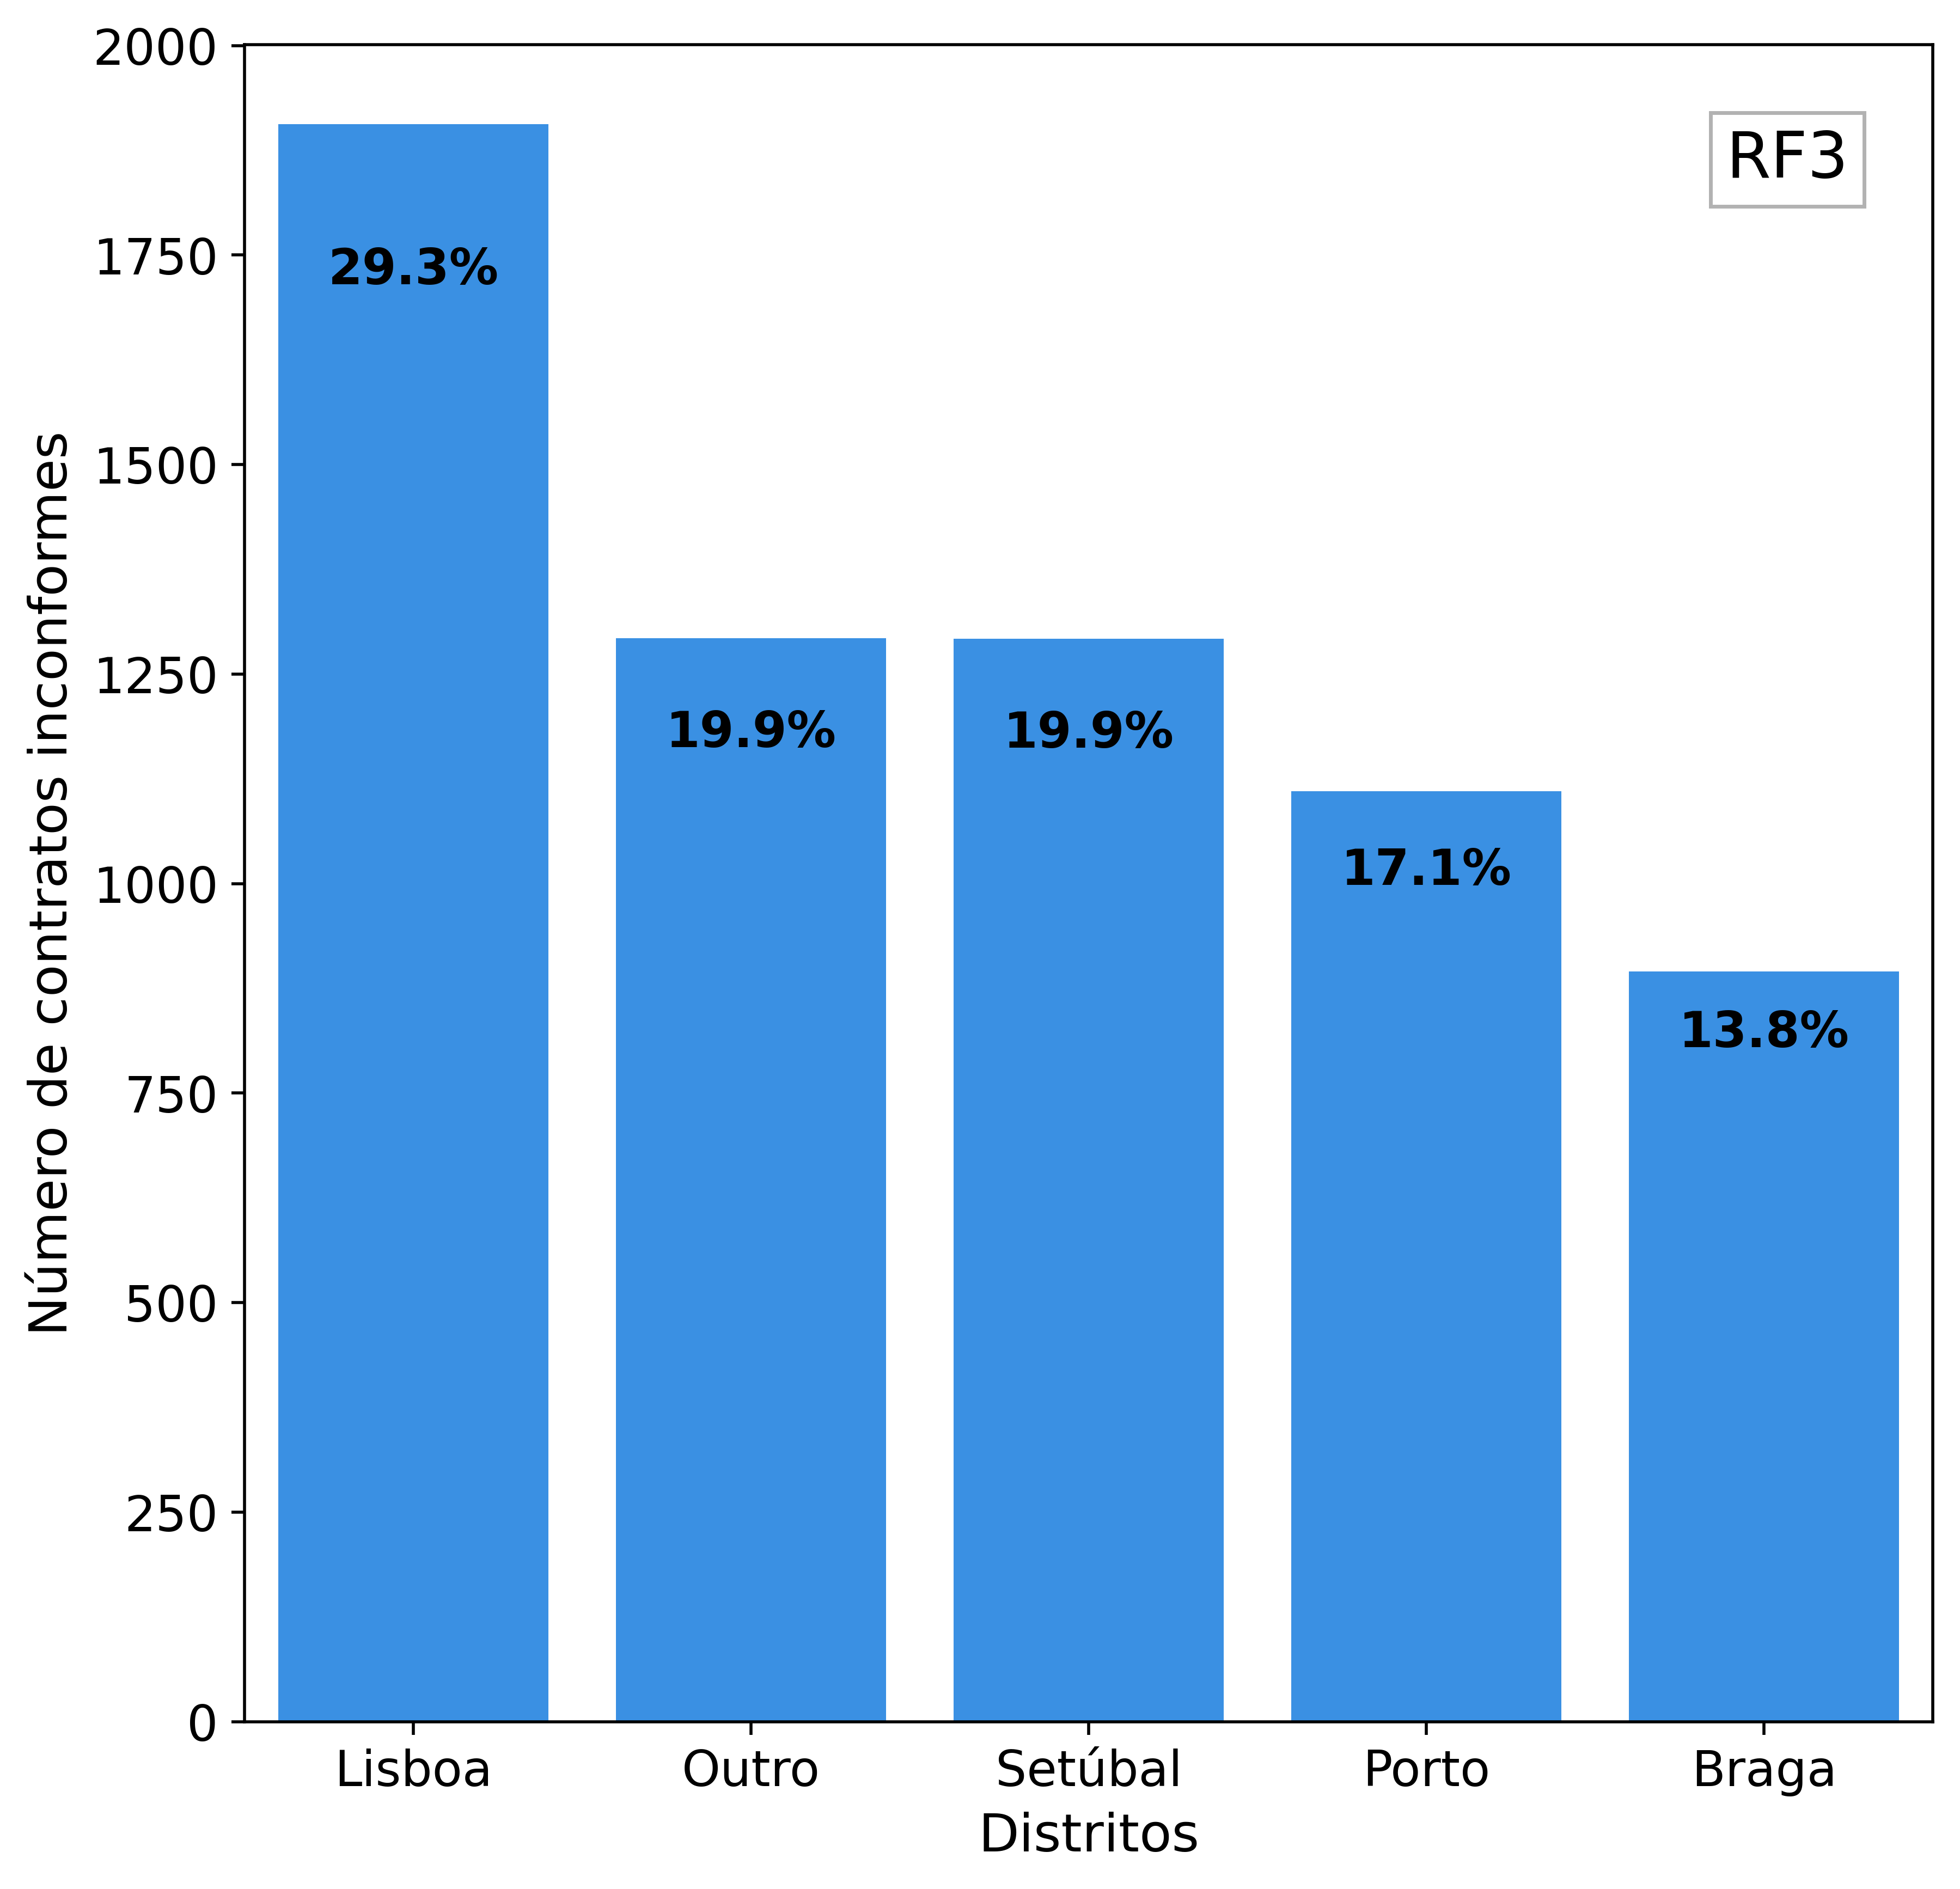
\includegraphics[width=\linewidth]{imagens/final/bar_RF3.png}
		\caption{Número de contratos sinalizados para o indicador RF3, por distrito.}
		\label{final11}
		
	\end{minipage}
\end{figure}


Por fim, fez-se uma contabilização do número de \textit{flags} detetadas por contrato. A Tabela \ref{final12} evidencia que, em 65565 (50.4\%) dos contratos analisados, no período de tempo considerado, não foi detetada nenhuma inconformidade. Por conseguinte, detetaram-se 39386 (30.3\%) e 20589 (15.8\%) contratos celebrados com uma e duas inconformidades em simultâneo, respetivamente. À medida que o número de flags ativadas em simultâneo aumenta, o número de contratos sinalizados diminui. 

\begin{table}[ht]
	\centering
	\renewcommand{\arraystretch}{1.5}
	\setlength{\tabcolsep}{15pt}
	\resizebox{\textwidth}{!}{
	\begin{tabular}{cccccccc}
		\toprule
		\textbf{Número de flags}       & 0     & 1     & 2     & 3    & 4   & 5      & 6 \\ \hline
		\textbf{\begin{tabular}[c]{@{}c@{}}Número de \\ contratos detetados \end{tabular}} & 65565 & 39386 & 20589 & 5794 & 587 & 21     & 0 \\ 
		\midrule
		\textbf{Percentagem \%}                                                             & 50.4  & 30.3  & 15.8  & 4.5  & 0.5 & $<0.5$ & 0 \\ \bottomrule
	\end{tabular}%
	}
	\caption{Número de contratos, com um número variável de flags ativadas em simultâneo, sinalizados.}
	\label{final12}
\end{table}


Na Tabela \ref{tab:resumofinal} encontram-se sintetizados os resultados para cada uma das flags aplicadas no processo de automação e para cada uma das principais divisões do CPV. Para cada divisão do CPV é mostrado o número total de contratos sinalizados, a fração de contratos no universo de contratos sinalizados, indepedentemente da divisão do CPV, e a percentagem de contratos sinalizados face ao número de contratos celebrados para a respetiva divisão do CPV.




\begin{table}[ht]
	\centering
	\renewcommand{\arraystretch}{1.5}
	\setlength{\tabcolsep}{10pt}
	\resizebox{\textwidth}{!}{
		
	\begin{tabular}{c|
			>{\columncolor[HTML]{EFEFEF}}c 
			>{\columncolor[HTML]{EFEFEF}}c 
			>{\columncolor[HTML]{EFEFEF}}c ccc
			>{\columncolor[HTML]{EFEFEF}}c 
			>{\columncolor[HTML]{EFEFEF}}c 
			>{\columncolor[HTML]{EFEFEF}}c ccc
			>{\columncolor[HTML]{EFEFEF}}c 
			>{\columncolor[HTML]{EFEFEF}}c 
			>{\columncolor[HTML]{EFEFEF}}c }
		\hline
		\textbf{Divisão CPV}                                                                  & \multicolumn{3}{c}{\cellcolor[HTML]{EFEFEF}45} & \multicolumn{3}{c}{33}                                                                     & \multicolumn{3}{c}{\cellcolor[HTML]{EFEFEF}15} & \multicolumn{3}{c}{90} & \multicolumn{3}{c}{\cellcolor[HTML]{EFEFEF}79} \\ \hline
		\textbf{\begin{tabular}[c]{@{}c@{}}Número total\\ contratos sinalizados\end{tabular}} & 24862         & 37.4\%         & 32.4\%        & \cellcolor[HTML]{FFFFFF}22379 & \cellcolor[HTML]{FFFFFF}33.7\%  & \cellcolor[HTML]{FFFFFF}6.8 & 3897          & 5.9\%         & 10.8\%         & 3554  & 5.4\% & 13.7\% & 3649          & 5.5\%          & 5.1\%         \\ \hline
		\cellcolor[HTML]{C0C0C0}\textbf{Flag}                                                 & \multicolumn{15}{c}{\cellcolor[HTML]{C0C0C0}}                                                                                                                                                                                                                          \\ \hline
		RF3                                                                                   & 3504          & 5.3\%          & 4.6\%         & 2263                          & 3.4\%                        & 0.7\%                       & 1070          & 1.6\%         & 3.0\%          & 571   & 0.9\% & 2.2\%  & 334           & 0.5\%          & 0.5\%         \\ \hline
		R003                                                                                  & 2898          & 4.4\%          & 3.8\%         & 336                           & 0.5\%                        & 0.1\%                       & 103           & 0.2\%         & 0.3\%          & 79    & 0.1\% & 0.3\%  & 91            & 0.1\%          & 0.1\%         \\ \hline
		R017                                                                                  & 6128          & 9.2\%          & 8.0\%         & 5446                          & 8.2\%                        & 1.6\%                       & 917           & 1.4\%         & 2.5\%          & 878   & 1.3\% & 3.4\%  & 1509          & 2.3\%          & 2.1\%         \\ \hline
		R018                                                                                  & 3546          & 5.3\%          & 4.6\%         & 4538                          & 6.8\%                        & 1.4\%                       & 1651          & 2.5\%         & 4.6\%          & 729   & 1.1\% & 2.8\%  & 832           & 1.3\%          & 1.2\%         \\ \hline
		R019                                                                                  & 8786          & 13.2\%         & 11.4\%        & 9796                          & 14.8\%                       & 3.0\%                       & 156           & 0.2\%         & 0.4\%          & 1297  & 2.0\% & 5.0\%  & 883           & 1.3\%          & 1.2\%         \\ \hline
	\end{tabular}%
		
	}
	\caption{Resumo do número total de contratos sinalizados, por categoria do CPV, e respetivos valores percentuais face ao número total de flags detetadas (independentemente da divisão do CPV) e número total de contratos celebrados por divisão de CPV, respetivamente. }
	\label{tab:resumofinal}
\end{table}



\begin{figure}[H]
	\centering
	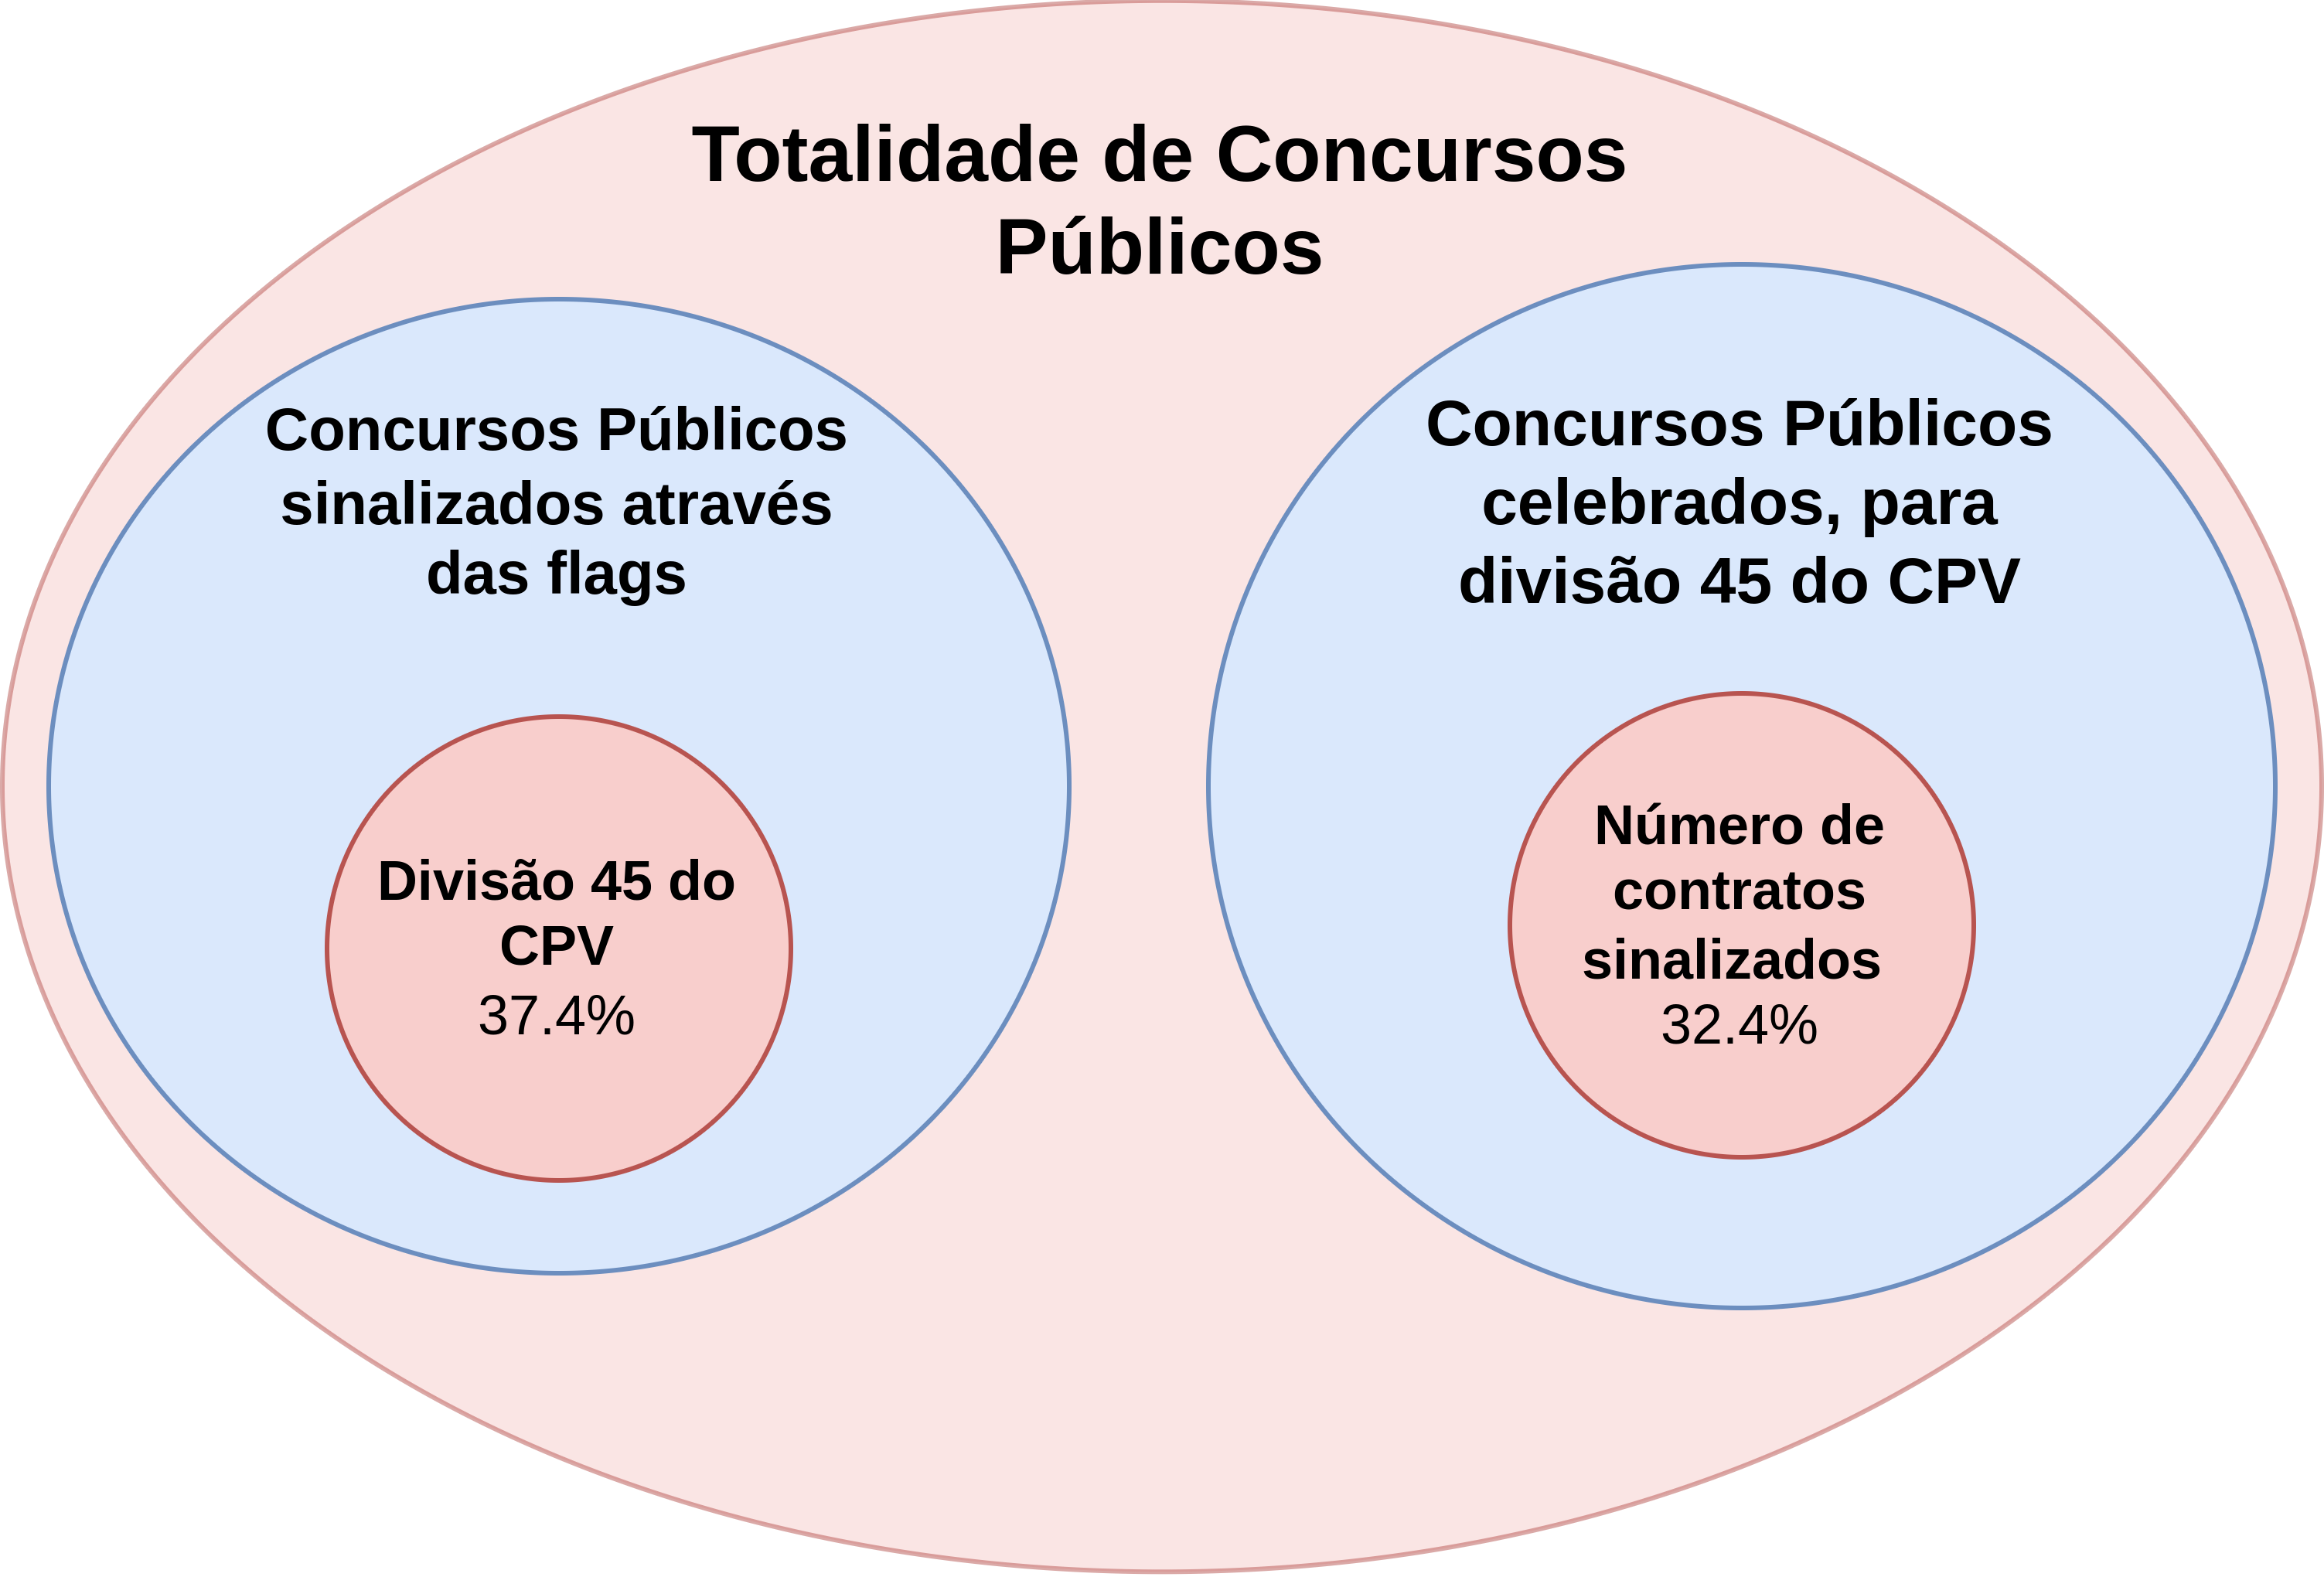
\includegraphics[width=0.6\textwidth]{imagens/final/confusao.png}
	\caption{Exemplo de ilustração dos valores total e percentuais, para a divisão 45 do CPV, passível de observar na Tabela \ref{tab:resumofinal}.}
	\label{}
\end{figure}








